%%%%%%%%%%%%%%%%%%%%%%%%%%%%%%%%%%%%%%%%%%%%%%%%%%%%%%%
% (19-12-2011) ~ MONOGRAFIA                           %
% DIOGO CEZAR TEIXEIRA BATISTA                        %
% ADAPTA��ES DO MODELO UFPR PARA DISSERTA��ES E TESES %
%%%%%%%%%%%%%%%%%%%%%%%%%%%%%%%%%%%%%%%%%%%%%%%%%%%%%%%

\documentclass[12pt,a4paper]{ufpr}

\usepackage[brazil]{babel}
\usepackage[latin1]{inputenc}
\usepackage[boxruled,noline,linesnumbered,portuguese,onelanguage,algoruled]{algorithm2e}
\usepackage[T1]{fontenc}
\usepackage{amssymb,amsmath}
\usepackage{multirow}
\usepackage{indentfirst}
\usepackage{amssymb}
\usepackage{subfigure}
\usepackage{graphicx}
\usepackage{caption2}
\usepackage{setspace}
\usepackage{longtable}
\usepackage{sty/ps-macros}
\usepackage{listings}
\usepackage{type1ec}
\usepackage{pdflscape}
\usepackage{color}
\usepackage{textcomp}
\usepackage{sty/ufpr}
\usepackage{acronym}

%%%%%%%%%%%%%%%%%
% CONFIGURA��ES %
%%%%%%%%%%%%%%%%%

\setcounter{secnumdepth}{3}
\setcounter{tocdepth}{3}

\lstset{numbers=left, stepnumber=1, firstnumber=1,
numberstyle=\scriptsize, extendedchars=true, breaklines=true,frame=tb,
basicstyle=\scriptsize, stringstyle=\scriptsize, showstringspaces=false}

\definecolor{listinggray}{gray}{0.9}
\definecolor{lbcolor}{rgb}{1,1,1}

\lstset{
	backgroundcolor=\color{lbcolor},
	tabsize=4,
	rulecolor=,
	language=matlab,
    basicstyle=\scriptsize,
    upquote=true,
    aboveskip={1.5\baselineskip},
    columns=fixed,
    showstringspaces=false,
    extendedchars=true,
    breaklines=true,
    prebreak = \raisebox{0ex}[0ex][0ex]{\ensuremath{\hookleftarrow}},
    frame=single,
    showtabs=false,
    showspaces=false,
    showstringspaces=false,
    identifierstyle=\ttfamily,
}

\renewcommand{\lstlistingname}{C�digo}
\renewcommand{\lstlistlistingname}{Lista de C�digos}

%%%%%%%%
% CAPA %
%%%%%%%%
%\title{T�cnicas de Planejamento para Gera��o de Planos de Execu��o em um Sistema Gerenciador de Fluxos de Trabalho Cient�fico}
\title{Um Modelo de Execu��o de Fluxos de Trabalho Cient�fico Utilizando T�cnicas de Planejamento Autom�tico}
\author{Diogo Cezar Teixeira Batista}
\advisortitle{Orientador} 
\advisorname{Prof. Dr. Fabiano Silva}
\advisorplace{Departamento de Inform�tica, UFPR}
\city{Curitiba}
\year{2012}
\banca
{Prof. Dr. }{Departamento de Inform�tica, UFPR}
{Prof. Dr. }{Departamento de Inform�tica, UFPR} 
{}{}
{}{}
\defesa{}

%%%%%%%%%%%%%
% DOCUMENTO %
%%%%%%%%%%%%%

\begin{document}

%%%%%%%%%%%%%%%
% PRE-TEXTUAL %
%%%%%%%%%%%%%%%

\makecapadissertacao
\makerosto
%\maketermo

%%%%%%%%%%%%%%%%
% ESPA�AMENTOS %
%%%%%%%%%%%%%%%%

%\singlespacing
%\onehalfspacing
\doublespacing

%%%%%%%%%%%%%%%%%%%%%%%
% ESTILO DA PAGINA��O %
%%%%%%%%%%%%%%%%%%%%%%%

\pagestyle{headings}
\pagenumbering{roman}

%%%%%%%%%%%%%%%%
% DEDEICAT�RIA %
%%%%%%%%%%%%%%%%

%\UFPRdedicatoria{Aos meus pais,      \\
A minha irm�,       \\
A minha orientadora.
}

%%%%%%%%%%%%%%%%%%
% AGRADECIMENTOS %
%%%%%%%%%%%%%%%%%%

%\UFPRagradecimentos{Agrade�o aos meus familiares em especial o mais pr�ximos, minha m�e querida Isabel Cristina Jos� Teixeira Batista, meu pai Mario Sergio Batista e a minha irm� Mayra Cristina Teixeira Batista, que me apoiaram e me confortaram nos �rduos momentos que enfrentei. Agrade�o a eles tamb�m pela oportunidade da plena dedica��o aos estudos, ajudando com meus custos at� conclus�o do curso.

Agrade�o a meu orientador, professor e amigo Fabiano Silva, que teve a paci�ncia e a dedica��o de me mostrar que na vida, os atalhos levam a trabalhos duplicados.

Agrade�o a meu amigo Ailton Sergio Bonifacio, que foi meu co-orientador no trabalho de conclus�o.

Agrade�o a meu amigo Guilherme Galante, que me ajudou muito em momentos cr�ticos nas disciplinas e no trabalho de conclus�o. 

Agrade�o a meu amigo Robson Gomes de Melo que estudou comigo por muitas horas teorias sobre grafos.

Agrade�o a meu professor e amigo Andr� Luiz Pires Guedes pelas tardes de discuss�es sobre teorias de algoritmos e grafos.

Agrade�o a meu amigo Jo�o Eug�nio, que me ajudou com as configura��es do PeerUnit.

Agrade�o as meu amigos Marcos Schreiner, Ronaldo Almeida e a todos os integrantes do laborat�rio LIAMF.

Gostaria de agradecer a todos os professores e colegas de trabalho da UTFPR que sempre me apoiaram e me incentivaram a cursar o mestrado.

Por fim, gostaria de agradecer a todos que de forma direta ou indireta colaboraram de alguma forma para o sucesso deste trabalho e para o meu sucesso.
}

%%%%%%%%%%%%%%%%%%%
% E P � G R A F E %
%%%%%%%%%%%%%%%%%%%

%\UFPRepigrafe{Your work is going to fill a large part of your life, and the only way to be truly satisfied is to do what you believe is great work. And the only way to do great work is to love what you do. If you haven't found it yet, keep looking, and don't settle. As with all matters of the heart, you'll know when you find it.}{Steve Jobs}

%%%%%%%%%%%
% SUM�RIO %
%%%%%%%%%%%

\tableofcontents

%%%%%%%%%%%%%%%%%%%%
% LISTA DE FIGURAS %
%%%%%%%%%%%%%%%%%%%%

\UFPRlistadefiguras

%%%%%%%%%%%%%%%%%%%%
% LISTA DE TABELAS %
%%%%%%%%%%%%%%%%%%%%

\UFPRlistadetabelas

%%%%%%%%%%%%%%%%%%%%
% LISTA DE CODIGOS %
%%%%%%%%%%%%%%%%%%%%

\UFPRlistadecodigos

%%%%%%%%%%%%%%%%%%%
% LISTA DE SIGLAS %
%%%%%%%%%%%%%%%%%%%

\UFPRlistadesiglas{\begin{acronym}
	\acro{BPEL4WS}[BPEL]{\emph{The Business Process Execution Language for Web Services}}
	\acro{DPLL}{\emph{Davis-Putnam-Logemann-Loveland}}
	\acro{FF}{\emph{Fast-Forward}}
	\acro{HSP}{\emph{Heuristic Search Planning}}
	\acro{IA}{Intelig�ncia Artificial}
	\acro{IPC4}{\emph{The 4th International Planning Competition}}
	\acro{MDS}{\emph{Globus Monitoring and Discovery Service}}
	\acro{MoML}{\emph{Modeling Markup Language}}
	\acro{ms}{Milisegundos}
	\acro{P2P}{\emph{Peer to Peer}}
	\acro{PDDL}{\emph{Planning Domain Definition Language}}
	\acro{RLS}{\emph{Globus Replica Location Service}}
	\acro{SAT}{Satisfabilidade}
	\acro{STRIPS}{\emph{STranford Research Institute Problem Solver}}
	\acro{SWEP}{\emph{Smart Workflow Execution by Planning}}
	\acro{TC}{\emph{Transformation Catalog}}
	\acro{VDL}{\emph{Virtual Data Language}}
	\acro{XML}{\emph{eXtensible Markup Language}}
\end{acronym}}

%%%%%%%%%%
% RESUMO %
%%%%%%%%%%

\UFPRresumo[Planejamento, Intelig�ncia Artificial, Fluxo de Trabalho Cient�fico, Computa��o Distribu�da]{
Experimentos cient�ficos produzem grande quantidade de informa��es que necessitam de processamento para uma posterior an�lise. Um cientista, que n�o � da �rea da computa��o, nem sempre possui as habilidades para desenvolver seu pr�prio ambiente de testes. Por isso a utiliza��o de executores de fluxos de trabalhos cient�ficos v�m sido largamente estudada. Uma das principais vantagens de se utilizar um processador de fluxo de trabalho cient�fico � a transpar�ncia oferecida para o cientista em rela��o a maneira com que os experimentos ser�o organizados, distribu�dos e processados. Este trabalho prop�e um modelo para cria��o de um ambiente que seja capaz de processar esses fluxos de trabalho. A �nfase est� em um escalonamento inteligente que utiliza t�cnicas para resolu��o de problemas de planejamento da �rea de intelig�ncia artificial.
}

%%%%%%%%%%%%
% ABSTRACT %
%%%%%%%%%%%%

\UFPRabstract[Planning, Artificial Intelligence, Scientific Workflow, Distributed Computing]{
Scientific experiments produce a large amount of information that require processing for further analysis. A scientist, that not work in computing area, does not always have the skills to develop their own test environment. Therefore the usage of executors of scientific workflows have been widely studied. The main advantage in use a workflow scientific processor is the transparency offered for the scientist regarding the manner in which the experiments will be organized, distributed and processed. This work proposes a model for creating an environment that be able to process these workflows. The emphasis is on a intelligent schedule that uses techniques to solve planning problems in the area of artificial intelligence.
}

%%%%%%%%%%%%%%%%%%%%%%%%%
% SEPARA��O DE PALAVRAS %
%%%%%%%%%%%%%%%%%%%%%%%%%

\hyphenation{F�-bri-ca-De-Pla-nos-De-Exe-cu-��o}

%%%%%%%%%%%%%%%%%%%%%%%
% ESTILO DA PAGINA��O %
%%%%%%%%%%%%%%%%%%%%%%%

\pagenumbering{arabic}

%%%%%%%%%%%%%
% CAP�TULOS %
%%%%%%%%%%%%%

%todo:

%defini��o n�vens

%melhorar custos

\section[Introdu��o]{Introdu��o}
\begin{frame}
    \frametitle{Introdu��o}
    \begin{itemize}

        \item <1-> Onde est� a p�gina que procuro em um site?

%        \item <1-> Grande n�mero de sistemas hiperm�dia;
%
%        \item <2-> Informa��es distribu�das desorganizadamente na Internet;
%
%        \item <3-> Sistemas de busca;
%
%            \begin{itemize}
%                \item <4-> Trazem conte�do n�o relacionado, ou
%                irrelevante (sem�ntica);
%                \item <5-> N�o oferecem assist�ncia navegacional;
%            \end{itemize}

        \item <2-> \emph{Hiperm�dia Adaptativa}: modifica��o do conte�do
        \emph{web}.

        \item <3-> Proposta: navega��o colaborativa;

            \begin{itemize}
                \item <4-> Ajuda m�tua entre os usu�rios que
                estiverem navegando pelas mesmas p�ginas;

                \item <5-> Solu��o baseada na teoria do comportamento das
                formigas;
            \end{itemize}

    \end{itemize}
\end{frame}

\chapter{Revis�o Bibliogr�fica}
\label{revisao-bibliografica}

Neste cap�tulo discute-se os assuntos relacionados ao trabalho proposto. Na se��o \ref{workflow} est�o descritos os conceitos de Fluxo de Trabalho Cient�fico. A se��o \ref{proveniencia} discorre sobre Proveni�ncia de Dados. A se��o \ref{ambiente} introduz os conceitos de Grades e Computa��o em Nuvens. A se��o \ref{p2p} descreve as caracter�sticas das aplica��es \UFPRsigla{P2P}. A se��o \ref{planejamento} apresenta as considera��es sobre Planejamento. E finalmente, na se��o \ref{plan-consideracoes} est�o as considera��es sobre o cap�tulo.

\section{Fluxo de Trabalho Cient�fico}
\label{workflow}

Os experimentos cient�ficos necessitam de processamento e analise de seus dados, essa tarefa vem se tornando complexa e pode envolver muitas etapas que necessitam coordena��o e integra��o. Al�m disso, � necess�rio tratar a distribui��o de dados a fim de se obter um tempo de execu��o vi�vel destes fluxos de trabalho.

Para tratar os desafios dos experimentos cient�ficos, utiliza-se sistemas que tem como objetivo o foco na coordena��o, integra��o e distribui��o de dados. Desta forma o sistema � capaz de executar experimentos que sejam estruturados de acordo com um modelo. Os experimentos cient�ficos s�o modelados em fluxos de trabalho  (\emph{workflow}) cient�fico.

Um fluxo de trabalho cient�fico � o encapsulamento de informa��es que pode ser processado automaticamente em um fluxo de execu��o, gerenciado por um sistema dito sistema gerenciador de fluxos de trabalho cient�fico. Estes sistemas transmitem documentos, tarefas ou informa��es de um participante para outro atrav�s de a��es. Estas a��es trabalham de forma coordenada de acordo com as regras estabelecidas entre os participantes formando um plano de execu��o \cite{Deelman2009}. 

O processo de execu��o de um fluxo de trabalho cient�fico pode ser dividido em etapas, s�o elas: \emph{composi��o}, \emph{orquestra��o}, \emph{mapeamento} e \emph{execu��o} \cite{Deelman2009}. A figura \ref{fig:workflow_model} ilustra as etapas para execu��o de fluxos de trabalho cientifico.

\begin{figure}[ht]
    \centering
    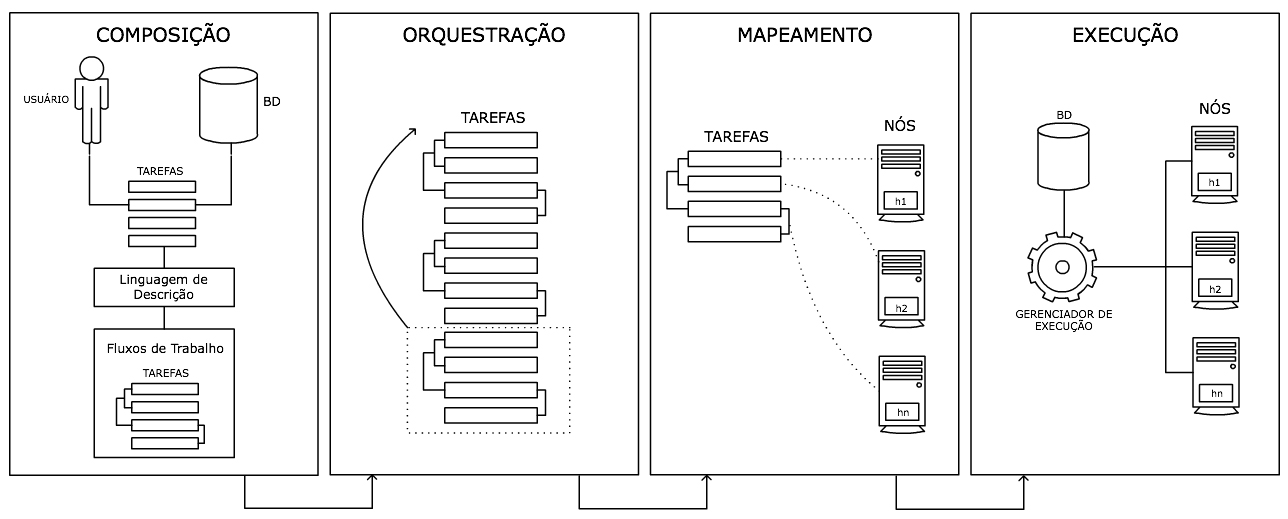
\includegraphics[width=16cm]{images/fig_workflow_model.jpg}
    \caption{Etapas para execu��o de fluxos de trabalho cient�fico}
    \label{fig:workflow_model}
\end{figure}

O processo de \emph{composi��o} de um fluxo de trabalho cient�fico est� relacionado � descri��o das tarefas que cada fluxo dever� executar, bem como a rela��o de depend�ncia entre elas. Normalmente sua representa��o � feita atrav�s de grafos dirigidos, no qual os v�rtices representam as tarefas e as arestas suas depend�ncias \cite{Deelman2009}.

Existem diversas linguagens para especifica��o de fluxo de trabalho cient�fico, cada qual com caracter�sticas distintas de sem�ntica, tipo de aplica��o, ambiente de execu��o ou representa��o \emph{abstrata} ou \emph{concreta}. Uma representa��o \emph{abstrata} n�o descreve os detalhes do ambiente execu��o. Uma representa��o \emph{concreta} descreve detalhes do ambiente de execu��o. Como exemplo de linguagens, apresenta-se: \UFPRsigla{MoML} \cite{Altintas2004}, \emph{Scufl} \cite{Belhajjame2008}, \emph{BPEL} \cite{Akram2006}, \UFPRsigla{VDL} \cite{Deelman2004} e \emph{DAX} \cite{Lee2008}. \UFPRsigla{MoML}, \emph{Scufl} e \emph{DAX}, s�o linguagens especificamente desenvolvidas para o processamento de fluxos de trabalho. \emph{BPEL} � uma linguagem para especificar a��es em processos de neg�cios dentro de servi�os \emph{web}, adaptada para execu��o de fluxos de trabalho. \emph{VDL} � uma linguagem utilizada para descri��o de dados utilizada pelo \emph{software} Chimera \cite{Foster2002}.

O processo de \emph{orquestra��o} tem como objetivo a coordena��o das tarefas que comp�em um fluxo de trabalho cient�fico. Outro objetivo � garantir que as depend�ncias sejam atendidas.

A etapa de \emph{mapeamento} tem como fun��o o escalonamento entre tarefas e recursos, para que um fluxo de trabalho seja execut�vel no ambiente de execu��o. Essa etapa pode ser feita com a interven��o do usu�rio, ou automaticamente atrav�s de um componente espec�fico. Em ambos os casos � necess�ria a obten��o de informa��es relativas aos recursos dispon�veis.

A \emph{execu��o} tem como fun��o a aloca��o e execu��o das tarefas nos n�s dispon�veis, al�m de tratar a toler�ncia a falhas e adaptabilidade dos fluxos de trabalho. A toler�ncia a falhas deve prever a realoca��o das tarefas de forma autom�tica caso um dos n�s seja desconectado. A adaptabilidade diz respeito a modelagem do fluxo de trabalho durante a execu��o. Isso se deve pela necessidade da varia��o dos dados de entrada espec�fica de cada aplica��o.

O modelo de execu��o pode utilizar abordagens orientadas a dados, controle ou h�brido. Essas abordagens tratam as depend�ncias entre tarefas. O modelo orientado a dados recebe os dados de entrada, aplica as opera��es e fornece o dado de sa�da como resultado ou como entrada para outra tarefa. Ao se trabalhar um sistema de controle, o gerenciador de fluxo de trabalho utiliza sinais que indicam o in�cio ou t�rmino da execu��o de determinado conjunto de dados. Nesse caso os dados s�o transportados de alguma forma impl�cita, n�o especificada, fazendo com que o sistema controle apenas o fluxo no qual as tarefas s�o executadas. Os sistemas h�bridos utilizam a jun��o das duas abordagens.

Algumas implementa��es est�o detalhadas no cap�tulo \ref{trabalhos-relacionados}.

\section{Proveni�ncia de Dados}
\label{proveniencia}

A proveni�ncia de dados � uma t�cnica de analise de dados que ajuda a determinar a deriva��o hist�rica de um dado ou processo, partindo de sua fonte original \cite{Simmhan2005,Miles}. O uso da proveni�ncia pode auxiliar na an�lise da \emph{qualidade de dados}, utilizado para estabelecer a qualidade e/ou confiabilidade dos dados baseado nos dados originais e suas transforma��es. Ainda � poss�vel a utiliza��o de rastreamento de dados pela \emph{trilha de auditoria}, que busca determinar o uso de recursos e a detec��o de erros na gera��o de dados. A \emph{replica��o} fornece informa��es detalhadas da proveni�ncia possibilitando a repeti��o da deriva��o de dados, para gerar uma poss�vel replica��o. Com a \emph{atribui��o} � poss�vel estabelecer o direito do autor sobre a propriedade de um dado, e determinar sua responsabilidade em caso de dados incorretos. Com a t�cnica \emph{informacional} possibilita-se a consulta baseada no hist�rico de metadados para a descoberta de novos dados \cite{Simmhan2005}. 

%\begin{itemize}
%	\item \emph{qualidade de dados}: usado para estabelecer a qualidade e/ou confiabilidade dos dados baseado nos dados originais e suas transforma��es;
%	\item \emph{trilha de auditoria}: pode ser usado rastreamento de dados, determinar uso de recursos e detec��o de erros na gera��o de dados;
%	\item \emph{replica��o}: informa��es detalhadas da proveni�ncia podem repetir a deriva��o de dados, podendo gerar uma poss�vel replica��o;
%	\item \emph{atribui��o}: � poss�vel estabelecer o direito do autor sobre a propriedade de um dado, e determinar sua responsabilidade em caso de dados incorretos.
%	\item \emph{informacional}: � a consulta baseada no hist�rico de metadados para a descoberta de novos dados.
%\end{itemize}

No que diz respeito � representa��o da proveni�ncia, diferentes t�cnicas podem ser usadas. As duas principais s�o \emph{anota��o} e \emph{invers�o}. A \emph{anota��o} diz respeito ao armazenamento de informa��es coletadas sobre os dados e os processos. A \emph{invers�o} faz um rastreamento de todo o processo de transforma��o dos dados, com intuito de tra�ar suas modifica��es \cite{Simmhan2005}. 

A t�cnica de \emph{anota��o} gera uma grande quantidade de metadados. O volume de metadados pode ficar maior que o pr�prio armazenamento de dados caso o m�todo de extra��o dos metadados seja detalhado. Por isso, a maneira de como a proveni�ncia ser� armazenada � importante para a escalabilidade. Quanto a forma de armazenamento, muitos sistemas de proveni�ncia utilizam a linguagem \UFPRsigla{XML} para represent�-los \cite{Miles}.

Em \cite{Miles2007}, s�o abordados casos de uso que justificam a utiliza��o de proveni�ncia em um ambiente cient�fico. Estes ilustram situa��es em que as t�cnicas de proveni�ncia de dados resolveriam problemas recorrentes do ambiente cient�fico, como por exemplo, um caso de uso que descreve uma situa��o na qual um cientista deseja registrar uma patente para os resultados de seu experimento, mas ao revisar o experimento um outro cientista percebe que o experimento possui restri��es legais e n�o pode ser patenteado. De acordo com um hist�rico de experimentos referenciados o cientista que ir� validar o experimento foca suas aten��es as restri��es legais, que passa desapercebido pelo cientista que deseja a patente.

%Bom base nos exemplos descritos por \cite{Miles2007}, prop�e-se um m�dulo para a valida��o de execu��o de fluxos de trabalho. Esta valida��o baseia-se em um documento de proveni�ncia que armazena resultados dos experimentos. A proveni�ncia cont�m o registro de todos as invoca��es dos servi�os, para que seja poss�vel a reprodu��o exata daquele experimento. Uma interface para publica��o de metadados permite que sejam adicionadas anota��es aos servi�os, agregando informa��es e detalhes para as pr�ximas execu��es. Sua estrutura permite que o usu�rio construa um fluxo de trabalho, e os envie para um m�quina que decide quais ser�o as tarefas que ir�o ser executadas. Ent�o, invoca-se os servi�os para a execu��o das tarefas na ordem correta. A cada execu��o as informa��es coletadas sobre o experimento repopulam o banco de metadados.

\section{Ambiente de Execu��o Distribu�do}
\label{ambiente}

Um ambiente distribu�do envolve a coordena��o e o compartilhamento dos recursos computacionais, armazenamento de dados e recursos de rede. 

%Uma grade computacional, � uma abordagem da �rea da computa��o distribu�da que envolve a coordena��o e o compartilhamento dos recursos computacionais, armazenamento de dados e recursos de rede atrav�s de distribui��es din�micas e geograficamente dispersas \cite{Sharma2010}.

Segundo \cite{Sharma2010}, o modelo b�sico de uma grade computacional � geralmente composto por um determinado n�mero de n�s, cada um contendo v�rios recursos computacionais. O agrupamento desses n�s pode ser classificado como \emph{homog�neos} ou \emph{heterog�neos}. Quando uma grade � homog�nea os recursos dispon�veis apresentam as mesmas caracter�sticas, enquanto que em uma grade heterog�nea os n�s apresentam caracter�sticas diferentes.

Destacam-se quatro componentes b�sicos em um modelo de grade:

\begin{itemize}
	\item \emph{usu�rio}: respons�vel por alimentar a grade com tarefas a serem processadas;
	\item \emph{gerenciador de recursos}: respons�vel por gerenciar a distribui��o das tarefas para os n�s, al�m de obter e utilizar informa��es do \emph{servi�o de informa��es da grade};
	\item \emph{servi�o de informa��es da grade}: captura informa��es sobre a execu��o dos n�s, que ajuda no processo de escalonamento;
	\item \emph{recursos da grade}: reuni�o dos n�s dispon�veis para processamento.
\end{itemize}

Quando um usu�rio necessita executar determinada tarefa essa solicita��o � enviada ao gerenciador de recursos, que com a ajuda do servi�o de informa��o da grade, escalona e distribui as tarefas. Cada n� processa a parte que lhe foi designada e retorna a tarefa processada para o gerenciador de recursos. O gerenciador de recursos junta as tarefas processadas e devolve o resultado para o usu�rio.

A Computa��o em Nuvens (do ingl�s \emph{Cloud Computing}) � um conceito de computa��o distribu�da que surgiu no meio comercial para oferecer servi�os e recursos na Internet espec�ficos para a necessidade dos usu�rios \cite{Armbrust2009}. Os aplicativos desenvolvidos para esse ambiente s�o desenvolvidos como um servi�o. Isso �, para extrair a informa��o do recurso na nuvem, deve-se adaptar o ambiente a um modelo de requisi��o e resposta. Para executar o servi�o, uma requisi��o com par�metros espec�ficos � enviada para a nuvem que processa as informa��es e retorna como resposta o processamento dos dados em quest�o.

A vantagem em utilizar os recursos como servi�os est� na instala��o, manuten��o e centraliza��o do controle de vers�es. Dessa forma os usu�rios podem usar o servi�o a qualquer hora, e de qualquer lugar.

Do ponto de vista dos recursos, a computa��o em nuvens pode oferecer tr�s novos aspectos:

\begin{enumerate}
	\item A possibilidade de recursos ``infinitos''. Na nuvem n�o existem limita��es de \emph{hardware}. Na teoria os recursos s�o flex�veis, limitados somente pelo provedor do recurso;
	\item Usu�rios da nuvem podem requisitar processamento de acordo com sua necessidade, e expandir o poder de processamento caso seja necess�rio;
	\item A capacidade de pagar pelos recursos por curtos prazos de utiliza��o, uma ou duas horas, conforme o necess�rio.
\end{enumerate}

\section{Sistemas Ponto a Ponto}
\label{p2p}

Sistemas \UFPRsigla{P2P} s�o sistemas distribu�dos, que consistem em n�s interconectados capazes de se auto-organizar em topologias de rede com o objetivo de compartilhar recursos, tais como: conte�do, ciclos de processamento, armazenamento e largura de banda. Estes sistemas s�o capazes de se adaptar a falhas e a acomoda��o transit�ria de n�s, sem a necessidade da intermedia��o ou suporte de um servidor centralizado \cite{Androutsellis-theotokis2004}. Segundo \cite{Androutsellis-theotokis2004}, existem duas caracter�sticas que definem uma arquitetura \UFPRsigla{P2P}:

\begin{enumerate}
	\item O compartilhamento de recursos de forma direta, sem a necessidade de um servidor centralizado. No entanto, sistemas que dependem da utiliza��o de um servidor centralizado para seu funcionamento b�sico (por exemplo, para a manuten��o de �ndices globais ou busca) se estendem a defini��o de \UFPRsigla{P2P}. Como os n�s de uma rede \UFPRsigla{P2P} n�o podem confiar em um servidor central para a coordena��o da troca de conte�do, eles s�o obrigados a participar ativamente de forma independente e unilateral realizando tarefas como: procura de n�s, localiza��o ou cache de conte�do, informa��es de roteamento, conex�o ou desconex�o de outros n�s vizinhos, sistema de criptografia e verifica��o de conte�do;
	\item Sua capacidade de tratar a instabilidade e conectividade como regras, adaptando-se automaticamente �s falhas de conex�o. Bem como uma popula��o transit�ria de n�s. Esta capacidade de auto-organiza��o tolerante a falhas necessita de uma topologia de rede adaptativa, que ir� mudar conforme a entrada ou sa�da de n�s, a fim de manter a sua conectividade e desempenho.
\end{enumerate}

Quanto � classifica��o proposta por \cite{Androutsellis-theotokis2004}, as aplica��es podem ser divididas em diferentes categorias descritas a seguir.

As aplica��es de \emph{Comunica��o e Colabora��o} incluem sistemas que oferecem uma infra-estrutura para facilitar a comunica��o direta e colaborativa entre computadores. Como exemplo est�o as aplica��es de troca de mensagens instant�neas e bate-papo.

%, como: \emph{Chat/Irc}, \emph{Instant Messaging} (Aol, Icq, Yahoo, Msn) e Jabber.

Nas aplica��es que envolvem \emph{Computa��o Distribu�da} est�o os sistemas que utilizam o processamento distribu�do dos n�s. Essa t�cnica distribui entre os n�s do sistema \UFPRsigla{P2P} pequenas tarefas para serem executadas, ao final do processamento executa-se um roteiro para coletar os resultados obtidos. Uma coordena��o central � invariavelmente necess�ria, principalmente para dividir, distribuir as tarefas e coletar os resultados.

Com aplica��es de \emph{Suporte a Servi�os de Internet} � poss�vel utilizar o ambiente \UFPRsigla{P2P} para compor um servi�o. Esse servi�o � utilizado como um componente que trabalha no modelo de requisi��o-resposta.

Aplica��es com \emph{Sistemas de Banco de Dados} podem utilizar a arquitetura \UFPRsigla{P2P} para constru��o de bancos de dados distribu�dos.

A \emph{Distribui��o de Conte�do} � a classifica��o mais comum para aplica��es \UFPRsigla{P2P}. Estas aplica��es incluem sistemas e infra-estruturas feitos para o compartilhamento de m�dia digital e outros dados entre os usu�rios.

O trabalho elaborado se enquadra na classifica��o \emph{Computa��o Distribu�da}, pois apresenta um sistema \UFPRsigla{P2P} como executor de tarefas de fluxos de trabalho cient�fico.

\section{Planejamento}
\label{planejamento}

%Nesse cap�tulo s�o apresentadas algumas considera��es iniciais sobre planejamento na se��o \ref{plan-introducao}. A se��o \ref{\UFPRsigla{PDDL}} descreve a linguagem \UFPRsigla{PDDL} utilizada para descri��o de problemas de planejamento. Nas se��es \ref{graphplan} e \ref{satplan} apresentam-se os trabalhos que inspiraram a evolu��o das t�cnicas de planejamento. Na se��o \ref{htn} apresenta-se uma outra t�cnica de planejamento. Na se��o \ref{crikey} � apresentado o planejador utilizado neste trabalho. E finalmente, na se��o \ref{plan-consideracoes} est�o as considera��es sobre o cap�tulo.

Problemas mapeados do mundo real podem apresentar um alto n�vel de complexidade. � dif�cil representar algumas caracter�sticas, como por exemplo: representa��o temporal, eventos inesperados e principalmente como estar� espa�o de estados depois de determinada modifica��o. Problemas que envolvam tais caracter�sticas est�o em uma classe de complexidade que se tornam invi�veis com algoritmos convencionais \cite{Weld1999}.

O planejamento em \UFPRsigla{IA} � uma t�cnica que busca tratar esse n�vel de complexidade de forma independente do dom�nio do problema. Nessa abordagem, ap�s o mapeamento detalhado do problema do mundo real, define-se um estado inicial conhecido e um estado final desejado. Para gerar um plano, elabora-se uma busca por um conjunto de a��es j� conhecidas, que modificam o cen�rio a cada execu��o. O desafio est� em encontrar em todo o espa�o de estados quais as a��es e em que ordem devem ser invocadas para gerar um plano v�lido para o problema de planejamento \cite{Weld1999}.

%A busca no espa�o de estados de um problema de planejamento � um problema que ficou em aberto durante muito tempo na �rea, pois qualquer tentativa de busca gerava uma quantidade exponencial de elementos a serem tratados. 

O \UFPRsigla{STRIPS} \cite{Fikes1971} foi o precursor dos planejamentos modernos. Com essa abordagem definiu-se a forma com que um problema e um dom�nio de planejamento s�o representados, e que � mantida na maioria dos planejadores atuais. Um \emph{estado} do problema � dado pelo conjunto de fatos verdadeiros em um determinado instante do plano. Um operador, ou a��o, � representado por:

\begin{itemize}
	\item \emph{pr�-condi��o}: s�o os requisitos necess�rios para que um determinado operador seja aplicado sobre um estado;
	\item \emph{lista de adi��o}: s�o os fatos a serem adicionados ao estado depois que operador � executado;
	\item \emph{lista de exclus�es}: s�o os efeitos negativos, ou seja, o conjunto de fatos que ser� retirado do estado ap�s a execu��o de um operador.
\end{itemize}

Um problema de planejamento � dado por dois conjuntos de fatos que representam o estado inicial e o estado final ou objetivo do problema, em um conjunto de operadores. Um plano, que � a solu��o para o problema de planejamento, � uma sequ�ncia de a��es que quando aplicada sobre o estado inicial obt�m o estado final do problema.

Quanto � classifica��o, os planejadores podem ser divididos em: \emph{cl�ssicos} ou \emph{hier�rquicos}. Os cl�ssicos executam uma busca no espa�o de estados com objetivo de encontrar um caminho (que representar� um conjunto de a��es) do estado inicial at� o estado objetivo. Os hier�rquicos utilizam uma t�cnica de decomposi��o de tarefas, dividindo uma tarefa complexa (abstrata) em uma ou mais tarefas com menor grau de complexidade (primitiva). Esse mapeamento � feito atrav�s de m�todos que descrevem poss�veis redu��es entre os operadores. 

%A classe de planejadores cl�ssicos � efetiva para a resolu��o de problemas com dom�nios relativamente pequenos e est�ticos, entretanto, falha ao tentar tratar dom�nios din�micos e mais complexos \cite{Porto2006}.

Outra classifica��o est� relacionada ao encadeamento, o encadeamento define como se dar� a busca no espa�o de estados. Um planejador pode possuir \emph{encadeamento para frente}, quando as a��es retornadas partem do estado inicial, ou \emph{encadeamento para traz}, quando as a��es retornadas partem do estado final \cite{Halsey2004,Coles}.

\subsection{Redes de Tarefas Hier�rquicas}
\label{htn}

Os planejadores \emph{hier�rquicos} s�o uma evolu��o dos cl�ssicos, e conseguem tratar uma gama de problemas com maior grau de complexidade pela infer�ncia direta de informa��es que refinam o processo de busca. Basicamente, a principal caracter�stica da abordagem hier�rquica est� na utiliza��o de a��es capazes de resolver subobjetivos que formam um objetivo maior \cite{Nau1999, Nau2003}. Essa infer�ncia de informa��es � feita atrav�s de \emph{m�todos}. Cada \emph{m�todo} � respons�vel por descrever quais a��es ou subtarefas ir�o compor uma tarefa mais complexa. Se uma tarefa � primitiva, ela n�o pode ser subdividida em uma tarefa menor, pois � poss�vel resolv�-la com as a��es j� descritas. O principal objetivo dessa abordagem � reduzir as tarefas complexas at� que existam somente tarefas primitivas, obtendo assim o plano \cite{Nau2003}. 

A maioria dos planejadores hier�rquicos s�o independentes do dom�nio, mas os m�todos, s�o espec�ficos do dom�nio. Isso faz com que seja necess�ria a a��o de um especialista para construir o dom�nio do problema, o que torna o planejador muito mais r�pido.

JSHOP2 \cite{Ilghami2006} � uma implementa��o de um planejador hier�rquico desenvolvida na linguagem Java. Seu desenvolvimento foi inspirado no planejador SHOP2 \cite{Nau2003}. O SHOP2 planeja as tarefas $T$ na mesma ordem que ser�o executadas. Para isso, uma escolha n�o-determin�stica de uma tarefa $t \in T$ que n�o possui predecessores, resulta em dois casos:

\begin{enumerate}
	\item se $t$ � primitivo, ent�o encontra-se uma a��o $a$ que resolve $t$ de forma que as pre-condi��es s�o satisfeitas em um estado $s$, e aplica $a$ em $s$. Se n�o existe essa a��o, ent�o esse ramo do espa�o de busca falha;
	\item se a tarefa $t$ � composta, ent�o o planejador encontra de forma n�o-determin�stica um m�todo $m$ que ir� decompor a tarefa $t$ em subtarefas. Se n�o existe um m�todo para tal decomposi��o, ent�o esse ramo do espa�o de busca falha.
\end{enumerate}

Se existe uma solu��o que envolve $m$, ent�o suas subtarefas far�o parte de uma nova lista atualizada $T'$ que � percorrida recursivamente at� que todas as tarefas sejam primarias e resolv�veis com operadores. 

As duas escolhas n�o-determin�stica presentes no algoritmo apresentado recaem inevitavelmente em um processo de busca exponencial \cite{Nau1999}.

No in�cio da elabora��o deste trabalho, os planejadores hier�rquicos foram foco dos estudos por apresentarem uma estrutura de resolu��o bastante semelhante a um fluxo de trabalho, que tamb�m pode ser hierarquicamente dividido. No ap�ndice \ref{jshop} apresenta-se um modelo inicial, constru�do com um planejador hiear�rquico. Entretanto notou-se que para extrair um plano paralelo do planejador em quest�o, seria necess�rio c�lculos de p�s-processamento, pois o planejador escolhido n�o era capaz de retornar planos paralelos. Por isso o \emph{CRIKEY} foi o planejador escolhido, descrito na se��o \ref{crikey}.

\subsection{Planejadores Cl�ssicos}

Em 1998, Daniel S. Weld \cite{Weld1999} fez um apanhado de duas principais t�cnicas que possibilitaram a retomada dos estudos em planejamento devido ao grande desempenho dos planejadores obtidos. Estes s�o exemplos de planejadores cl�ssicos, e est�o brevemente descritas a seguir.

A id�ia do \emph{Graphpan} \cite{Blum1995} � a representa��o do espa�o de estados atrav�s de um grafo. Nesse grafo existem dois tipos de v�rtices: \emph{proposi��o} e \emph{a��o}. A constru��o do grafo � feita de modo que os v�rtices estejam separados por camadas. As camadas pares s�o formadas por v�rtices de proposi��o enquanto que as camadas �mpares s�o compostas por v�rtices de a��es. A camada zero (inicial) � formada por proposi��es que representam os fatos do estado inicial do problema. Arestas ligam os v�rtices de proposi��es aos de a��es, cujas pr�-condi��es mencionam tais proposi��es ou que representam os efeitos das a��es.

A��es que est�o na mesma camada, podem ter uma caracter�stica de exclus�o m�tua, se uma for escolhida a outra n�o pode ser, devido a conflitos entre as pre-condi��es e os efeitos destas a��es. Nesse caso existem arestas que as conectam classificando-as como mutuamente exclusivos.

Para extrair a solu��o na estrutura definida, o planejador faz uma tentativa de gerar o plano com $n$ passos. Logo, � necess�ria a representa��o do grafo at� a camada $2n$, depois faz-se uma busca de encadeamento para traz, procurando um caminho que chegue ao estado inicial do problema. Se ao voltar pelo grafo, a��es mutuamente exclusivas s�o escolhidas, aplica-se a t�cnica de \emph{backtraking} at� que todas as op��es estejam esgotadas. Caso n�o se encontre um caminho com $n$ passos, o algoritmo expande o grafo para a camada $2(n+1)$ e realiza o procedimento novamente.

Baseados no grafo de planos proposto por \cite{Blum1995}, alguns planejadores direcionam os estudos para buscas heur�sticas. O planejador \UFPRsigla{FF} \cite{Hoffmann2002}, por exemplo, utiliza o grafo de planos e uma busca heur�stica baseada no \UFPRsigla{HSP} \cite{Bonet2001}. O \UFPRsigla{FF} realiza uma busca progressiva no espa�o de estados utilizando a t�cnica de \emph{subida de encosta refor�ada}. Essa t�cnica pode ser definida como: partindo de um estado $S$, avalia-se todos os seus sucessores diretos $S'$. Se nenhum deles tem uma heur�stica melhor que $S$, procure pelos sucessores dos sucessores, e assim sucessivamente at� encontrar um estado $S'$ com heur�stica melhor que $S$. O planejador \emph{CRIKEY} \cite{Halsey2004,Coles} � inspirado no planejador \UFPRsigla{FF} e est� detalhado na se��o \ref{crikey}.

\UFPRsigla{SAT} � um problema da \UFPRsigla{IA} que procura uma valora��o que torne uma f�rmula l�gica proposicional verdadeira. Inicialmente proposto por \cite{Kautz1992}, um planejador baseado em \UFPRsigla{SAT} tem como entrada um problema de planejamento que gera uma f�rmula l�gica proposicional, que se for satisfeita por alguma valora��o para suas vari�veis proposicionais, implica na exist�ncia de um plano, que pode ser obtido a partir de tal valora��o.

Ao traduzir o problema de planejamento para \UFPRsigla{SAT}, torna-se necess�rio um resolvedor \UFPRsigla{SAT} eficiente. Devido ao alto desempenho dos resolvedores \UFPRsigla{SAT} atuais, esta t�cnica de planejamento ainda � a que apresenta um melhor desempenho \cite{Kautz2006}.

%melhorar �ltimo par�grafo

%alto desempenho SAT = t�cnica apresenta melhor desempenho

%HSP, FF, MIPS, CRIKEY

%que podem ser classificados em \emph{sistem�ticos} ou \emph{estoc�sticos}. Resolvedores sistem�ticos s�o determin�sticos e normalmente utilizam o algoritmo \UFPRsigla{DPLL} para executar uma busca em profundidade, com recurso de \emph{backtraking}. Os estoc�sticos n�o s�o determin�sticos, utilizam uma busca local usando movimenta��es aleat�rias, com objetivo de fugir da m�nima local. Essa abordagem, por ser incompleta, quando invocada para resolver problemas dif�ceis podem simplesmente responder que n�o foi poss�vel encontrar um resultado em tempo satisfat�rio.

Com o avan�o dos estudos na �rea de planejamento foi proposta a unifica��o da descri��o dos dom�nios e problemas em uma linguagem comum a v�rios planejadores, a linguagem \UFPRsigla{PDDL}.

\subsection{\emph{Planning Domain Definition Language}}
\label{pddl}

%Ap�s a identifica��o da necessidade da utiliza��o de um planejador que suportasse planos paralelos, bem como a utiliza��o de m�tricas, optou-se pela utiliza��o de planejadores que interpretassem a linguagem \UFPRsigla{PDDL} (\emph{Planning Domain Definition Language}).

A linguagem \UFPRsigla{PDDL} fornece uma base para a descri��o de problemas de planejamento, permitindo que os modelos possam ser compartilhados de forma padronizada entre a comunidade cient�fica. Em sua vers�o 2.1 a linguagem conta com defini��es para utiliza��o de dom�nios que tratem a��es com um tempo de dura��o, bem como a utiliza��o de m�tricas que permitem procurar por um plano espec�fico que busque maximizar ou minimizar o valor de uma vari�vel, que pode ser incrementada ou decrementada dependendo da a��o que � executada \cite{Fox2003}.

A linguagem \UFPRsigla{PDDL} � formada por:

\begin{itemize}
	\item \emph{objetos}: entidades representadas num problema de planejamento;
	\item \emph{predicados}: propriedades dos objetos;
	\item \emph{estado inicial}: � um conjunto de predicados sobre objetos que representam o estado do mundo quando o processo de planejamento � iniciado;
	\item \emph{objetivo}: � o conjunto de predicados que deve ser verdadeiro no estado final gerado pelo plano;
	\item \emph{a��es/operadores}: meios de mudar o estado do mundo.
\end{itemize}

As especifica��es em \UFPRsigla{PDDL} s�o separadas em dois arquivos: \emph{dom�nio} e \emph{problema}. O \emph{dom�nio} possui os predicados e as a��es. O \emph{problema} possui os objetos, o estado inicial e a especifica��o do objetivo.

Um arquivo de dom�nio tem a estrutura disposta no c�digo \ref{def_domain} e um arquivo de problema tem sua estrutura exemplificada no c�digo \ref{def_problem}.

\UFPRcode{Java}{def_domain}{Estrutura de um arquivo PDDL de dom�nio}{codes/def_domain.txt}

\UFPRcode{Java}{def_problem}{Estrutura de um arquivo PDDL de problema}{codes/def_problem.txt}

Para exemplificar a descri��o de um problema na linguagem \UFPRsigla{PDDL}, apresenta-se um problema cl�ssico da \UFPRsigla{IA} chamado \emph{mundo dos blocos}. Esse problema consiste basicamente de blocos sobre uma mesa e um bra�o mec�nico que movimenta os blocos. O objetivo � determinar um plano a partir de um estado inicial e um estado final. Os c�digos \ref{def_domain_blocks} e \ref{def_problem_blocks} representam o dom�nio e um problema do problema do mundo dos blocos.

\UFPRcode{Java}{def_domain_blocks}{Dom�nio exemplo: mundo de blocos}{codes/def_domain_blocks.txt}

\UFPRcode{Java}{def_problem_blocks}{Problema exemplo: mundo de blocos}{codes/def_problem_blocks.txt}

Na defini��o do dom�nio, s�o criados os predicados que ser�o utilizados para validar as poss�veis a��es. S�o elas: pegar um bloco, soltar um bloco, empilhar um bloco, desempilhar um bloco.

O problema � composto por 4 blocos $A, B, C$ e $D$ o estado inicial diz que todos os blocos est�o desempilhados, o bra�o mec�nico est� vazio e os 4 blocos est�o na mesa. O objetivo � ter $C$ sobre $D$, $B$ sobre $C$ e $A$ sobre $B$.

O plano gerado est� transcrito no c�digo \ref{plan_problem_blocks}.

\UFPRcode{Java}{plan_problem_blocks}{Plano gerado: mundo de blocos}{codes/plan_problem_blocks.txt}

No ap�ndice \ref{plan-files} encontram-se exemplos de especifica��es de problemas na linguagem \UFPRsigla{PDDL} utilizados neste trabalho.

%Os c�digos para as especifica��es \UFPRsigla{PDDL} s�o exemplificados no ap�ndice \ref{plan-files}.

\subsection{Crikey}
\label{crikey}

O \emph{CRIKEY} \cite{Halsey2004,Coles} � um planejador que utiliza uma heur�stica de busca com encadeamento para frente, baseada na m�trica \UFPRsigla{FF} \cite{Hoffmann2002}, implementado na linguagem Java, em sua vers�o 1.4. Ele � completo mas n�o � �timo (no tempo ou na m�trica especificada). Ele vai, entretanto, fazer uma tentativa para minimizar o n�mero de a��es em um plano.

O planejador foi escrito para trabalhar com os modelos de m�tricas e tempo da linguagem \UFPRsigla{PDDL} 2.1 \cite{Fox2003}. Ele � capaz de tratar ambos os aspectos temporais: a��es durativas e recursos de m�tricas. Nos dom�nios \UFPRsigla{PDDL}: \texttt{:typing}, \texttt{:fluents}, e \texttt{:durative-actions}.

\emph{CRIKEY} separa o planejamento do escalonamento das partes temporais do problema (no caso do planejamento temporal). A t�cnica utilizada busca detectar onde esses dois sub-problemas est�o fortemente acoplados, para separ�-los completamente. Depois que o planejador obt�m um plano totalmente ordenado, aplica-se a rede temporal, que gera como sa�da o plano temporal.

Durante o planejamento a informa��o temporal � ignorada. A estrat�gia de pesquisa � aplicada em subidas de encosta, ou seja, uma vez que o melhor estado � encontrado, a pesquisa continua daquele estado sem retrocesso. Se a busca por subida de encosta falha, retorna-se para o estado inicial, o que tecnicamente gera um novo plano. Assim como na t�cnica FF, somente as a��es �teis s�o consideradas. A��es �teis s�o a��es que aparecem na primeira camada do grafo de planejamento. \cite{Halsey2004}.

A utiliza��o do planejador � feita por um arquivo do tipo \emph{.jar} que recebe como par�metro tr�s arquivos: \emph{dom�nio}, \emph{problema} e \emph{sa�da}. Os arquivos de \emph{dom�nio} e \emph{problema} s�o constru��es definidas pela linguagem \UFPRsigla{PDDL}, e o arquivo de \emph{sa�da} possui um padr�o que disp�e as informa��es sobre a ordem de execu��o, a a��o utilizada e as proposi��es que comp�em essa a��o. De acordo com o modelo proposto, a integra��o com o planejador foi feita atrav�s da chamada externa de um comando que gera o arquivo de sa�da, que � utilizado para extrair as devidas informa��es necess�rias para dar seguimento ao fluxo de execu��o.

A utiliza��o de m�trica utilizada no modelo, diz respeito a procura por um plano que minimize o incremento de uma vari�vel. Esse incremento � feito com valores diferentes para cada uma das a��es do planejador, dessa forma, procura-se por um caminho que busque o menor custo, gerando assim um plano mais refinado e pr�ximo da solu��o �tima.

O \emph{CRIKEY} participou da competi��o \UFPRsigla{IPC4} realizada em 2004, onde obteve bons resultados.

\section{Considera��es}
\label{plan-consideracoes}

%workflow

Ao utilizar fluxos de trabalhos cient�ficos, os usu�rios podem focar suas aten��es em seus experimentos e deixar a complexidade de gerenciamento para o ambiente de execu��o. Atualmente, pela grande vantagem em se utilizar ambientes de nuvem, os projetos que utilizam esse ambiente tem destaque.

%proveniencia

Como quase sempre o objetivo principal de experimento cient�fico � a minimiza��o do tempo de execu��o, a utiliza��o de um coletor de informa��es sobre os recursos pode ser utilizado como um mecanismo de coleta de metadados. Com estas informa��es � poss�vel tra�ar um hist�rico da taxa de ocupa��o dos recursos e utiliz�-las para a obten��o de um plano refinado.

% ambientes distribu�dos

Independente do ambiente de execu��o (uma grade ou nuvem) ao se utilizar uma aplica��o baseada na estrutura \UFPRsigla{P2P} cada n� deve possuir as caracter�sticas para se manter de forma aut�noma na rede. Para a adapta��o de um modelo que utilize \emph{Computa��o Distribu�da} � necess�ria a modifica��o do ambiente para a utiliza��o de um n� central respons�vel por coletar os resultados processados. Quanto ao armazenamento de informa��es sobre a ocupa��o dos n�s, � necess�rio que cada n� seja indexado com um identificador. A utiliza��o de um sistema \UFPRsigla{P2P} e os detalhes modificados s�o apresentados na se��o \ref{peerunit}.

%planejamento

Quanto �s t�cnicas de planejamento, inicialmente optou-se pela utiliza��o de uma planejador hier�rquico. Isso pela similaridade da decomposi��o de um fluxo de trabalho e a decomposi��o de tarefas oferecida pelo planejador hier�rquico. Por exemplo, um fluxo de trabalho pode ser definido em $n$ subtarefas e cada subtarefa dividida em $n_i$ subsubtarefas. Entretanto, depois de um modelo inicial testado (ap�ndice \ref{jshop}), notou-se que para extrair um plano paralelo do planejador em quest�o, seria necess�rio c�lculos de p�s-processamento. Por permitir a execu��o de planos paralelos, ter sua implementa��o em Java e mostrar-se um planejador r�pido, o \emph{CRIKEY} foi adotado como planejador no modelo proposto. O \emph{CRIKEY} ainda utiliza a linguagem \UFPRsigla{PDDL} como entrada para resolu��o de seus problemas.

A vantagem ao se utilizar a linguagem \UFPRsigla{PDDL} colaborou diretamente para o desacoplamento do planejador. Se a implementa��o seguisse com a utiliza��o do \emph{JSHOP}, todo o tradutor teria que ser re-escrito caso fosse necess�ria a utiliza��o de outro planejador. Ao optar pela tradu��o para a linguagem \UFPRsigla{PDDL}, qualquer planejador que suporte a linguagem em sua vers�o 2.1 pode ser facilmente acoplado ao sistema. Aumentando assim a modularidade do sistema.

A escolha do planejamento para compor um plano de execu��o, tem potencialidade para fornecer tipos refinados de planos. A medida que se incrementa a possibilidade de parametriza��o na gera��o de um plano, planos mais espec�ficos podem ser gerados. Como por exemplo, tentar tra�ar um plano que minimize ao inv�s do tempo de execu��o, o consumo de energia. Isso � poss�vel atrav�s da infer�ncia de informa��es coletadas do pr�prio hist�rico de execu��es do modelo. Por esse motivo, a cria��o de um modelo que utilize t�cnicas de planejamento tem potencialidade para n�o s� escalonar de forma eficiente, mas tamb�m alterar o esquema de execu��o de acordo com a necessidade do usu�rio. A potencialidade da gera��o de planos de execu��o � discutida na se��o \ref{plan-custos}.
\section[Trabalhos Relacionados]{Trabalhos Relacionados}

\begin{frame}
    \frametitle{Trabalhos Relacionados}
    \begin{itemize}
		\item Ptolemy, 2003 e Kepler, 2004:
		\item Pegasus, 2004;
		\item SciCumulus, 2010;
		\item Dornemann, Juhnke, Noll, Seiler e Freisleben, 2010;
		\item Gil, Deelman, Blythe, Kesselman e Tangmunarunkit, 2004;
		\item Compara��es;
	\end{itemize}
\end{frame}

\begin{frame}
    \frametitle{Trabalhos Relacionados}
	\begin{itemize}
		\item Ptolemy/Kepler:
		\begin{itemize}
			\item implementa��o da mesma opera��o sobre dados de diferentes formas (atores);
			\item modelo � capaz de selecionar qual a melhor implementa��o do operador para a execu��o em quest�o;
		\end{itemize}
		\item Pegasus:
		\begin{itemize}
			\item sistema � realimentado com metadados coletados em suas execu��es;
		\end{itemize}
		\item SciCumulus:	
		\begin{itemize}
			\item inspirou a utiliza��o de paralelismo: sobre dados e sobre execu��o;
		\end{itemize}
	\end{itemize}
\end{frame}

\begin{frame}
    \frametitle{Trabalhos Relacionados e Compara��es}

	\begin{itemize}
		
		\item Dornemann at al, 2010:
		\begin{itemize}
			\item coletor de informa��es;
		\end{itemize}
		\item Gil at al, 2004:
		\begin{itemize}
			\item aprimora o escalonamento utilizando t�cnicas de planejamento;
		\end{itemize}
	\end{itemize}

	\scriptsize
	\begin{table}[!htb]
		\begin{tabular}{|l|l|l|l|l|}
		\cline{2-5}
		\multicolumn{1}{l|}{} & \multicolumn{1}{c|}{Ambiente} & \multicolumn{1}{c|}{Descri��o Fluxos} & \multicolumn{1}{c|}{Metadados} & \multicolumn{1}{c|}{Escalonamento} \\ 
		\hline
		Ptolemy & \multicolumn{1}{c|}{-} & \multicolumn{1}{c|}{-} & \multicolumn{1}{c|}{N�o} & \multicolumn{1}{c|}{Estrutura} \\ 
		\hline
		Kepler & \multicolumn{1}{c|}{-} & \multicolumn{1}{c|}{MoML} & \multicolumn{1}{c|}{N�o} & \multicolumn{1}{c|}{Estrutura} \\ 
		\hline
		Pegasus & \multicolumn{1}{c|}{Grade} & \multicolumn{1}{c|}{VDL} & \multicolumn{1}{c|}{Sim} & \multicolumn{1}{c|}{Condor-G} \\ 
		\hline
		SciCumulus & \multicolumn{1}{c|}{Nuvem} & \multicolumn{1}{c|}{VisTrails} & \multicolumn{1}{c|}{N�o} & \multicolumn{1}{c|}{VisTrails} \\ 
		\hline
		Dornemann at al, 2010 & \multicolumn{1}{c|}{Nuvem} & \multicolumn{1}{c|}{WS-BPEL} & \multicolumn{1}{c|}{N�o} & \multicolumn{1}{c|}{Algoritmo Gen�tico} \\ 
		\hline
		Gil at al, 2004 & \multicolumn{1}{c|}{Grade} & \multicolumn{1}{c|}{VDL} & \multicolumn{1}{c|}{Sim} & \multicolumn{1}{c|}{Planejamento} \\ 
		\hline
		\end{tabular}
	\end{table}
	\normalsize
\end{frame}

\section[Modelo Proposto - Smart Workflow Execution by Planning (SWEP)]{Modelo Proposto - Smart Workflow Execution by Planing (SWEP)}

\begin{frame}
    \frametitle{Proposta SWEP - \emph{Smart Workflow Execution by Planing}}
	\begin{itemize}
		\item Planejador (\emph{CRIKEY});
		\item Ambiente P2P (\emph{PeerUnit});
		\item Caracter�sticas:
		\begin{itemize}
			\item m�tricas flex�veis;
			\item t�cnicas de paraleliza��o;
			\item proveni�ncia e metadados;
		\end{itemize}
	\end{itemize}
\end{frame}

\begin{frame}
    \frametitle{Modelo Proposto - SWEP (\emph{Smart Workflow Execution by Planing})}
	\begin{itemize}
		\item vis�o geral;
		\item vis�o detalhada;
		\item paralelismos;
		\item m�tricas flex�veis;
		\item m�todo de tradu��o;
	\end{itemize}
\end{frame}

\begin{frame}
	\begin{changemargin}{-1cm}{-1cm}
	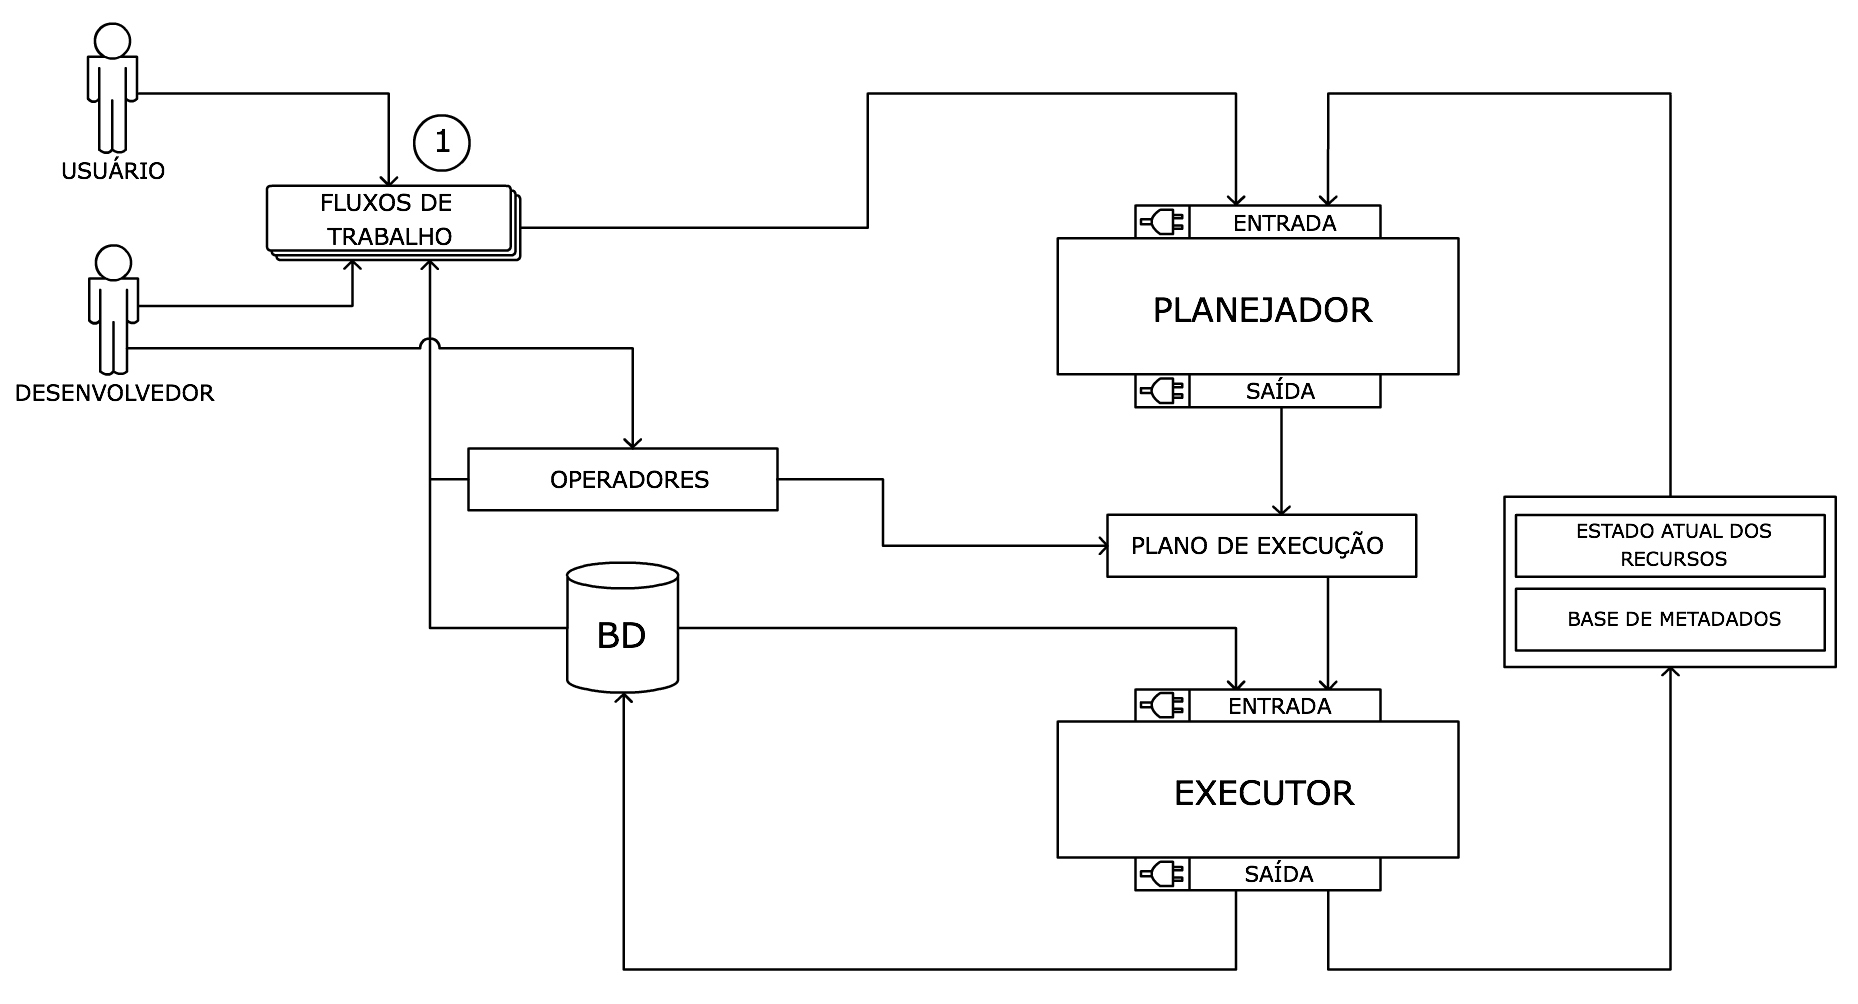
\includegraphics[width=12.8cm]{../images/fig_sys_overview-1.jpg}
	\end{changemargin}
\end{frame}

\begin{frame}
	\begin{changemargin}{-1cm}{-1cm}
	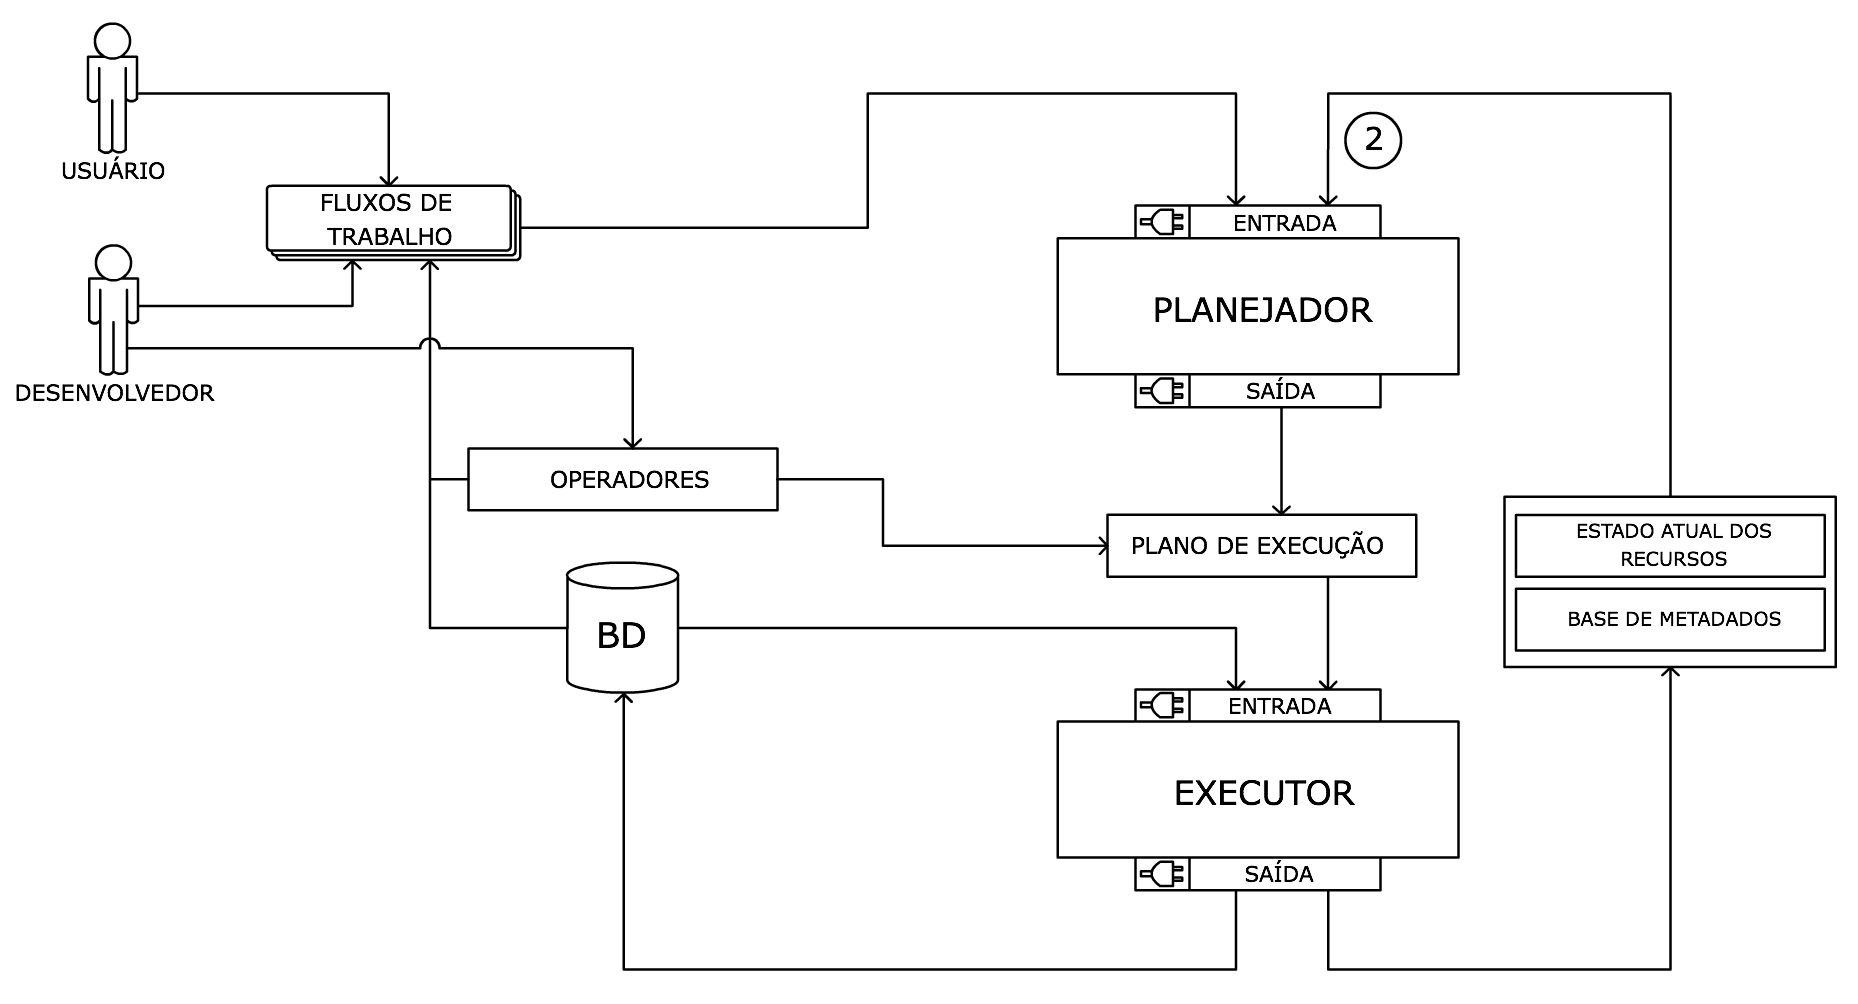
\includegraphics[width=12.8cm]{../images/fig_sys_overview-2.jpg}
	\end{changemargin}
\end{frame}

\begin{frame}
	\begin{changemargin}{-1cm}{-1cm}
	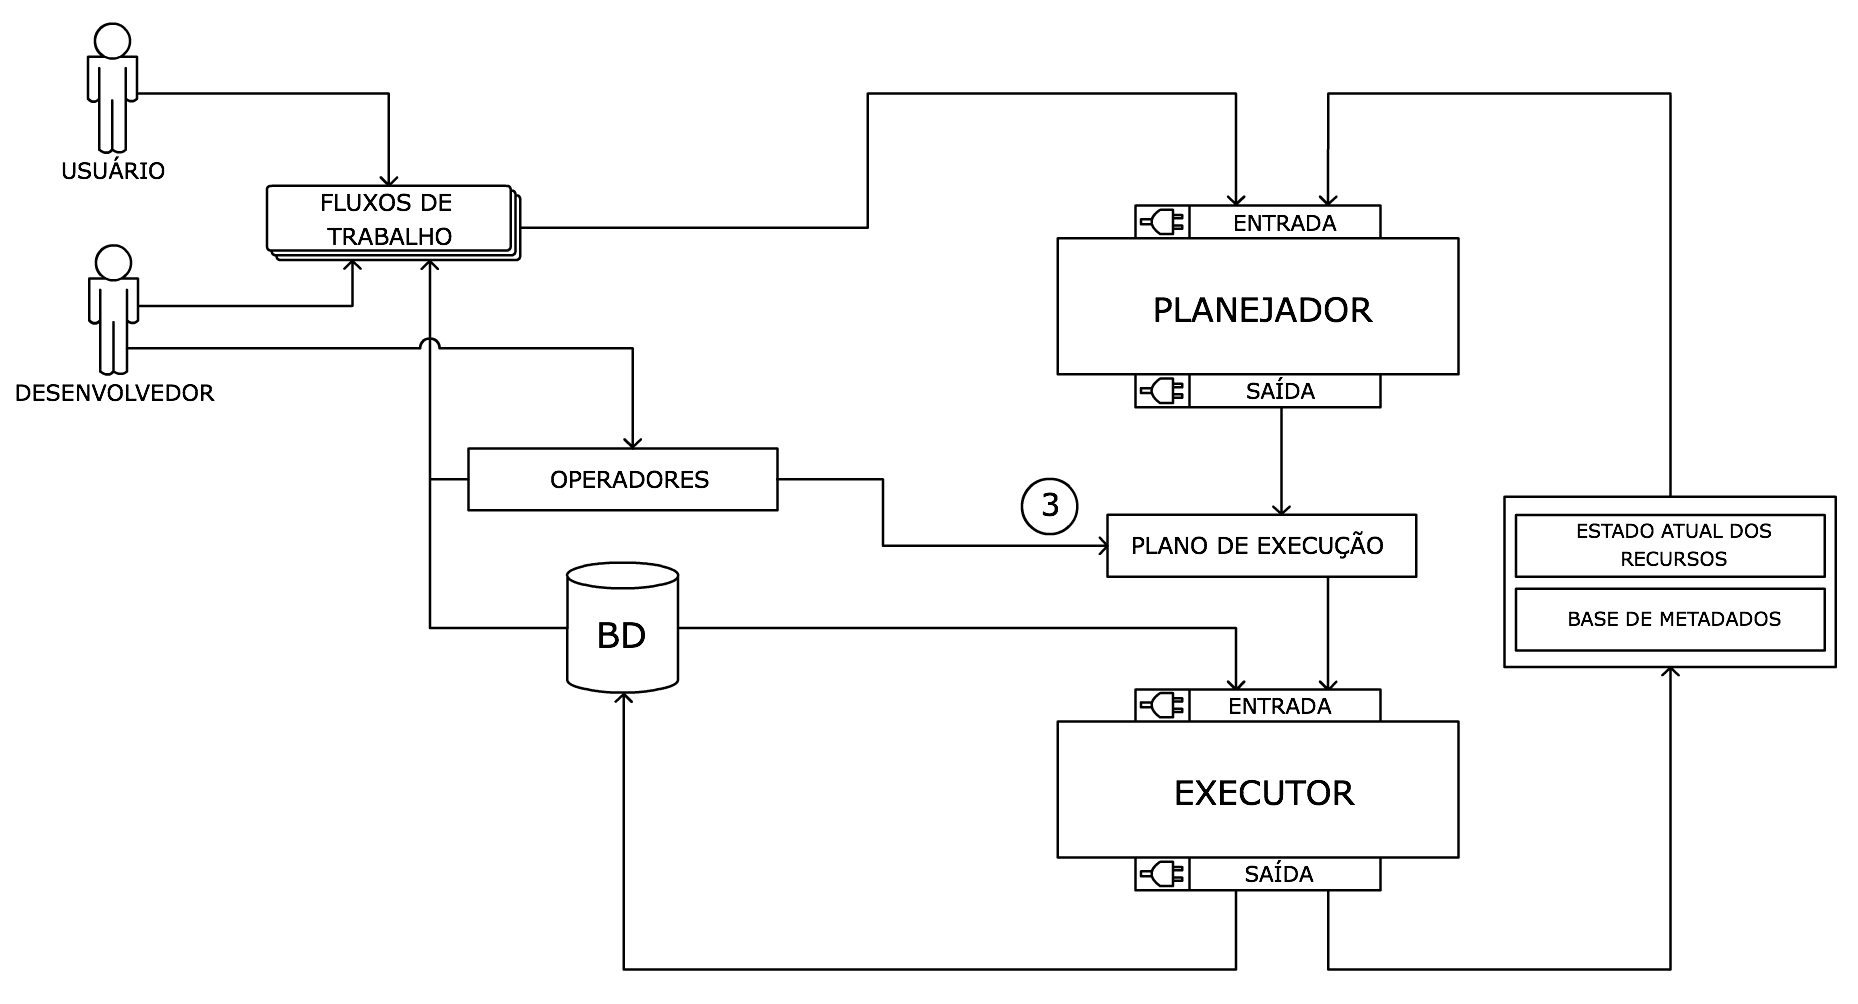
\includegraphics[width=12.8cm]{../images/fig_sys_overview-3.jpg}
	\end{changemargin}
\end{frame}

\begin{frame}
	\begin{changemargin}{-1cm}{-1cm}
	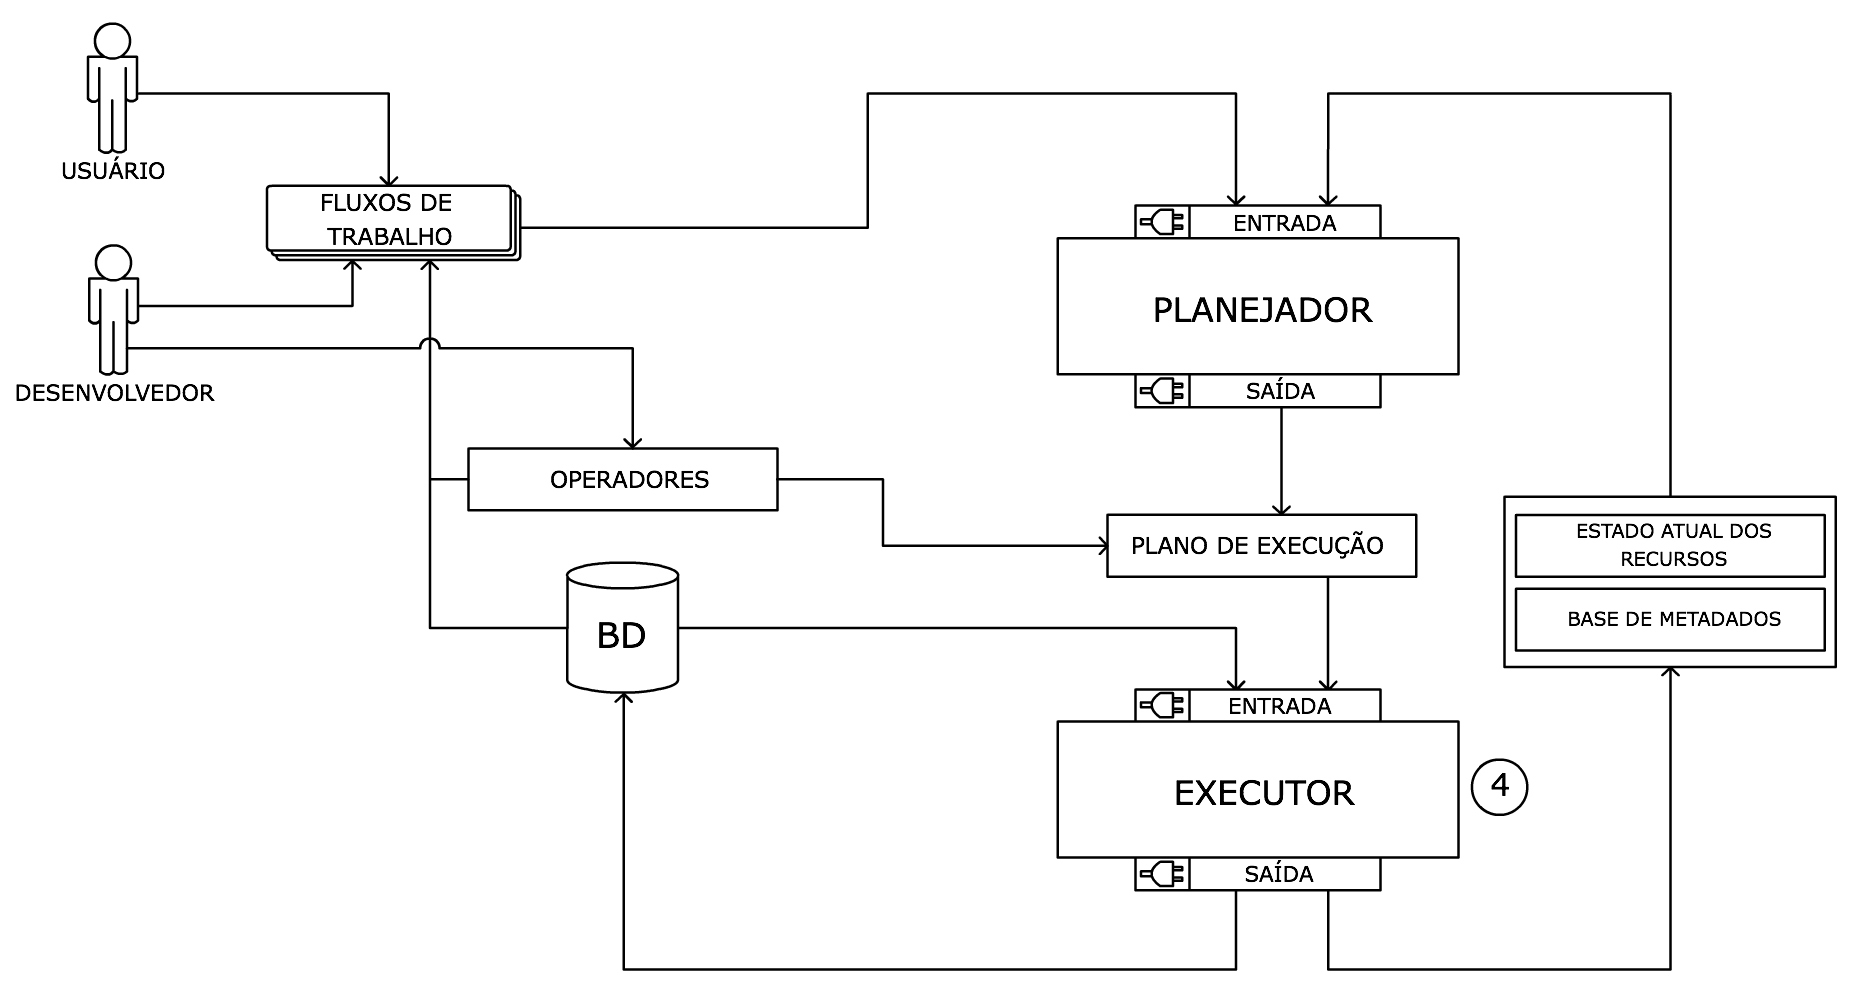
\includegraphics[width=12.8cm]{../images/fig_sys_overview-4.jpg}
	\end{changemargin}
\end{frame}

\begin{frame}
	\begin{changemargin}{-1cm}{-1cm}
	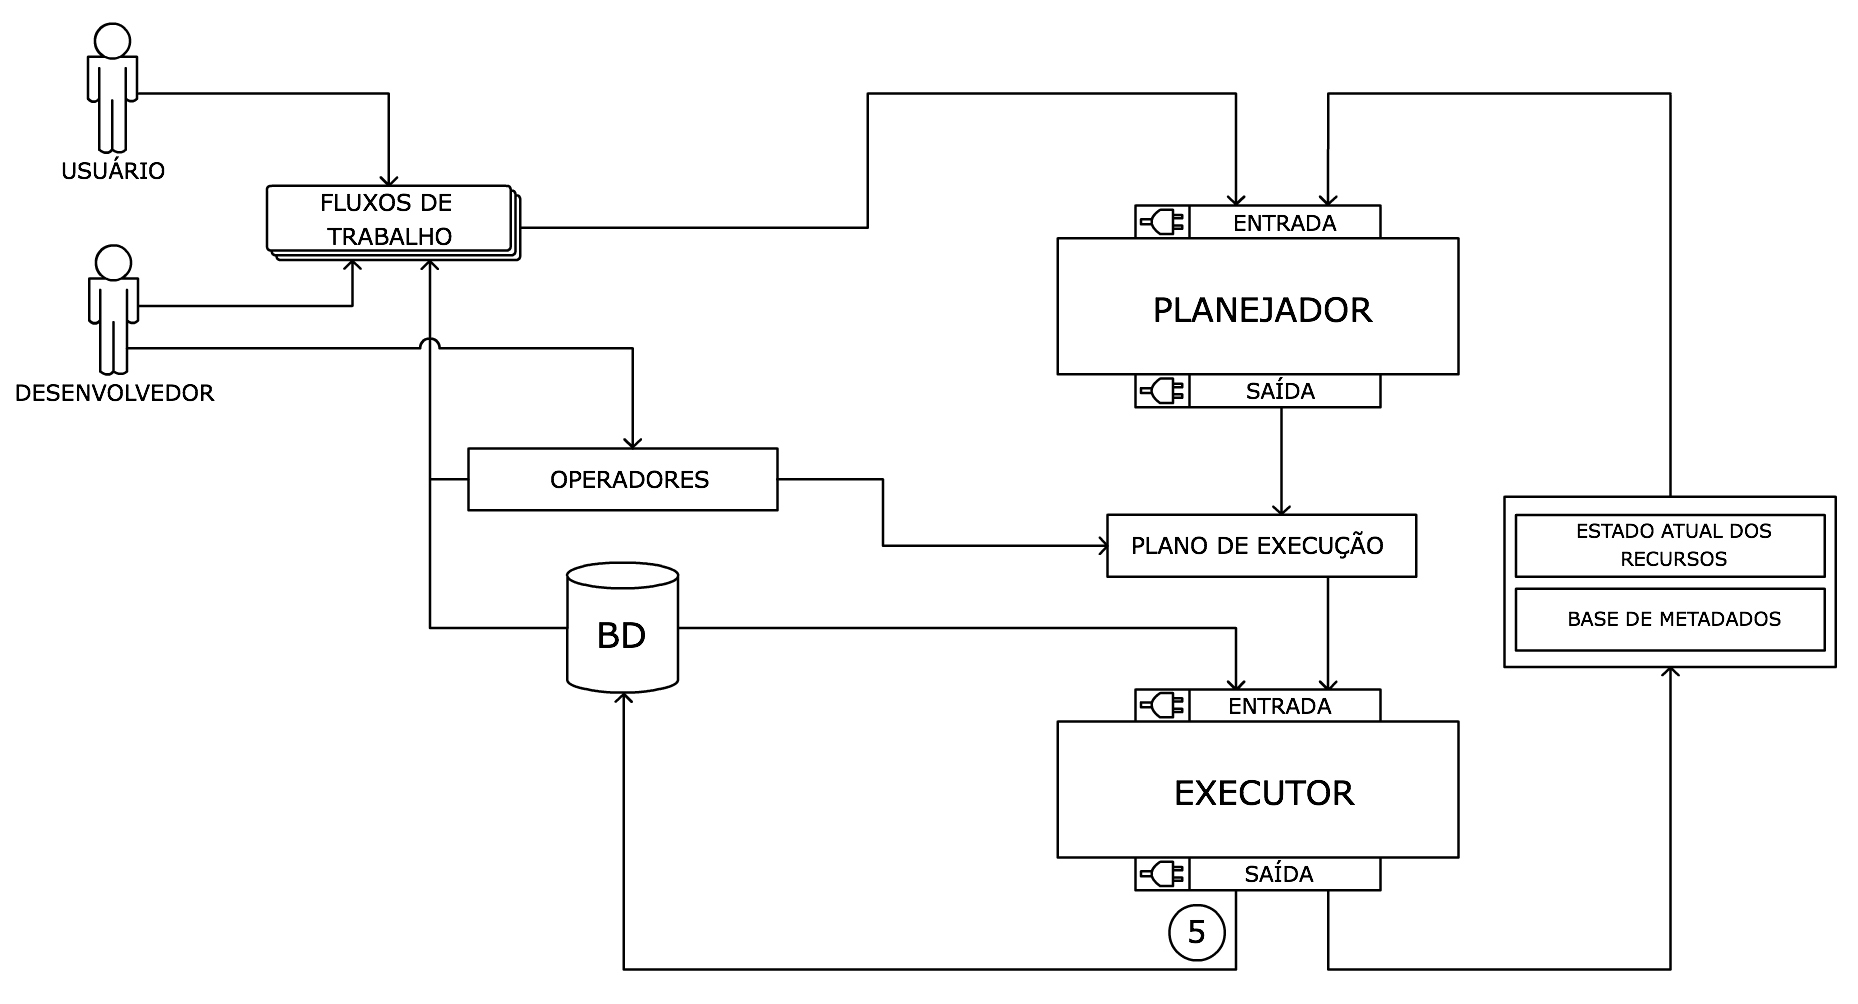
\includegraphics[width=12.8cm]{../images/fig_sys_overview-5.jpg}
	\end{changemargin}
\end{frame}

\begin{frame}
	\begin{changemargin}{-1cm}{-1cm}
	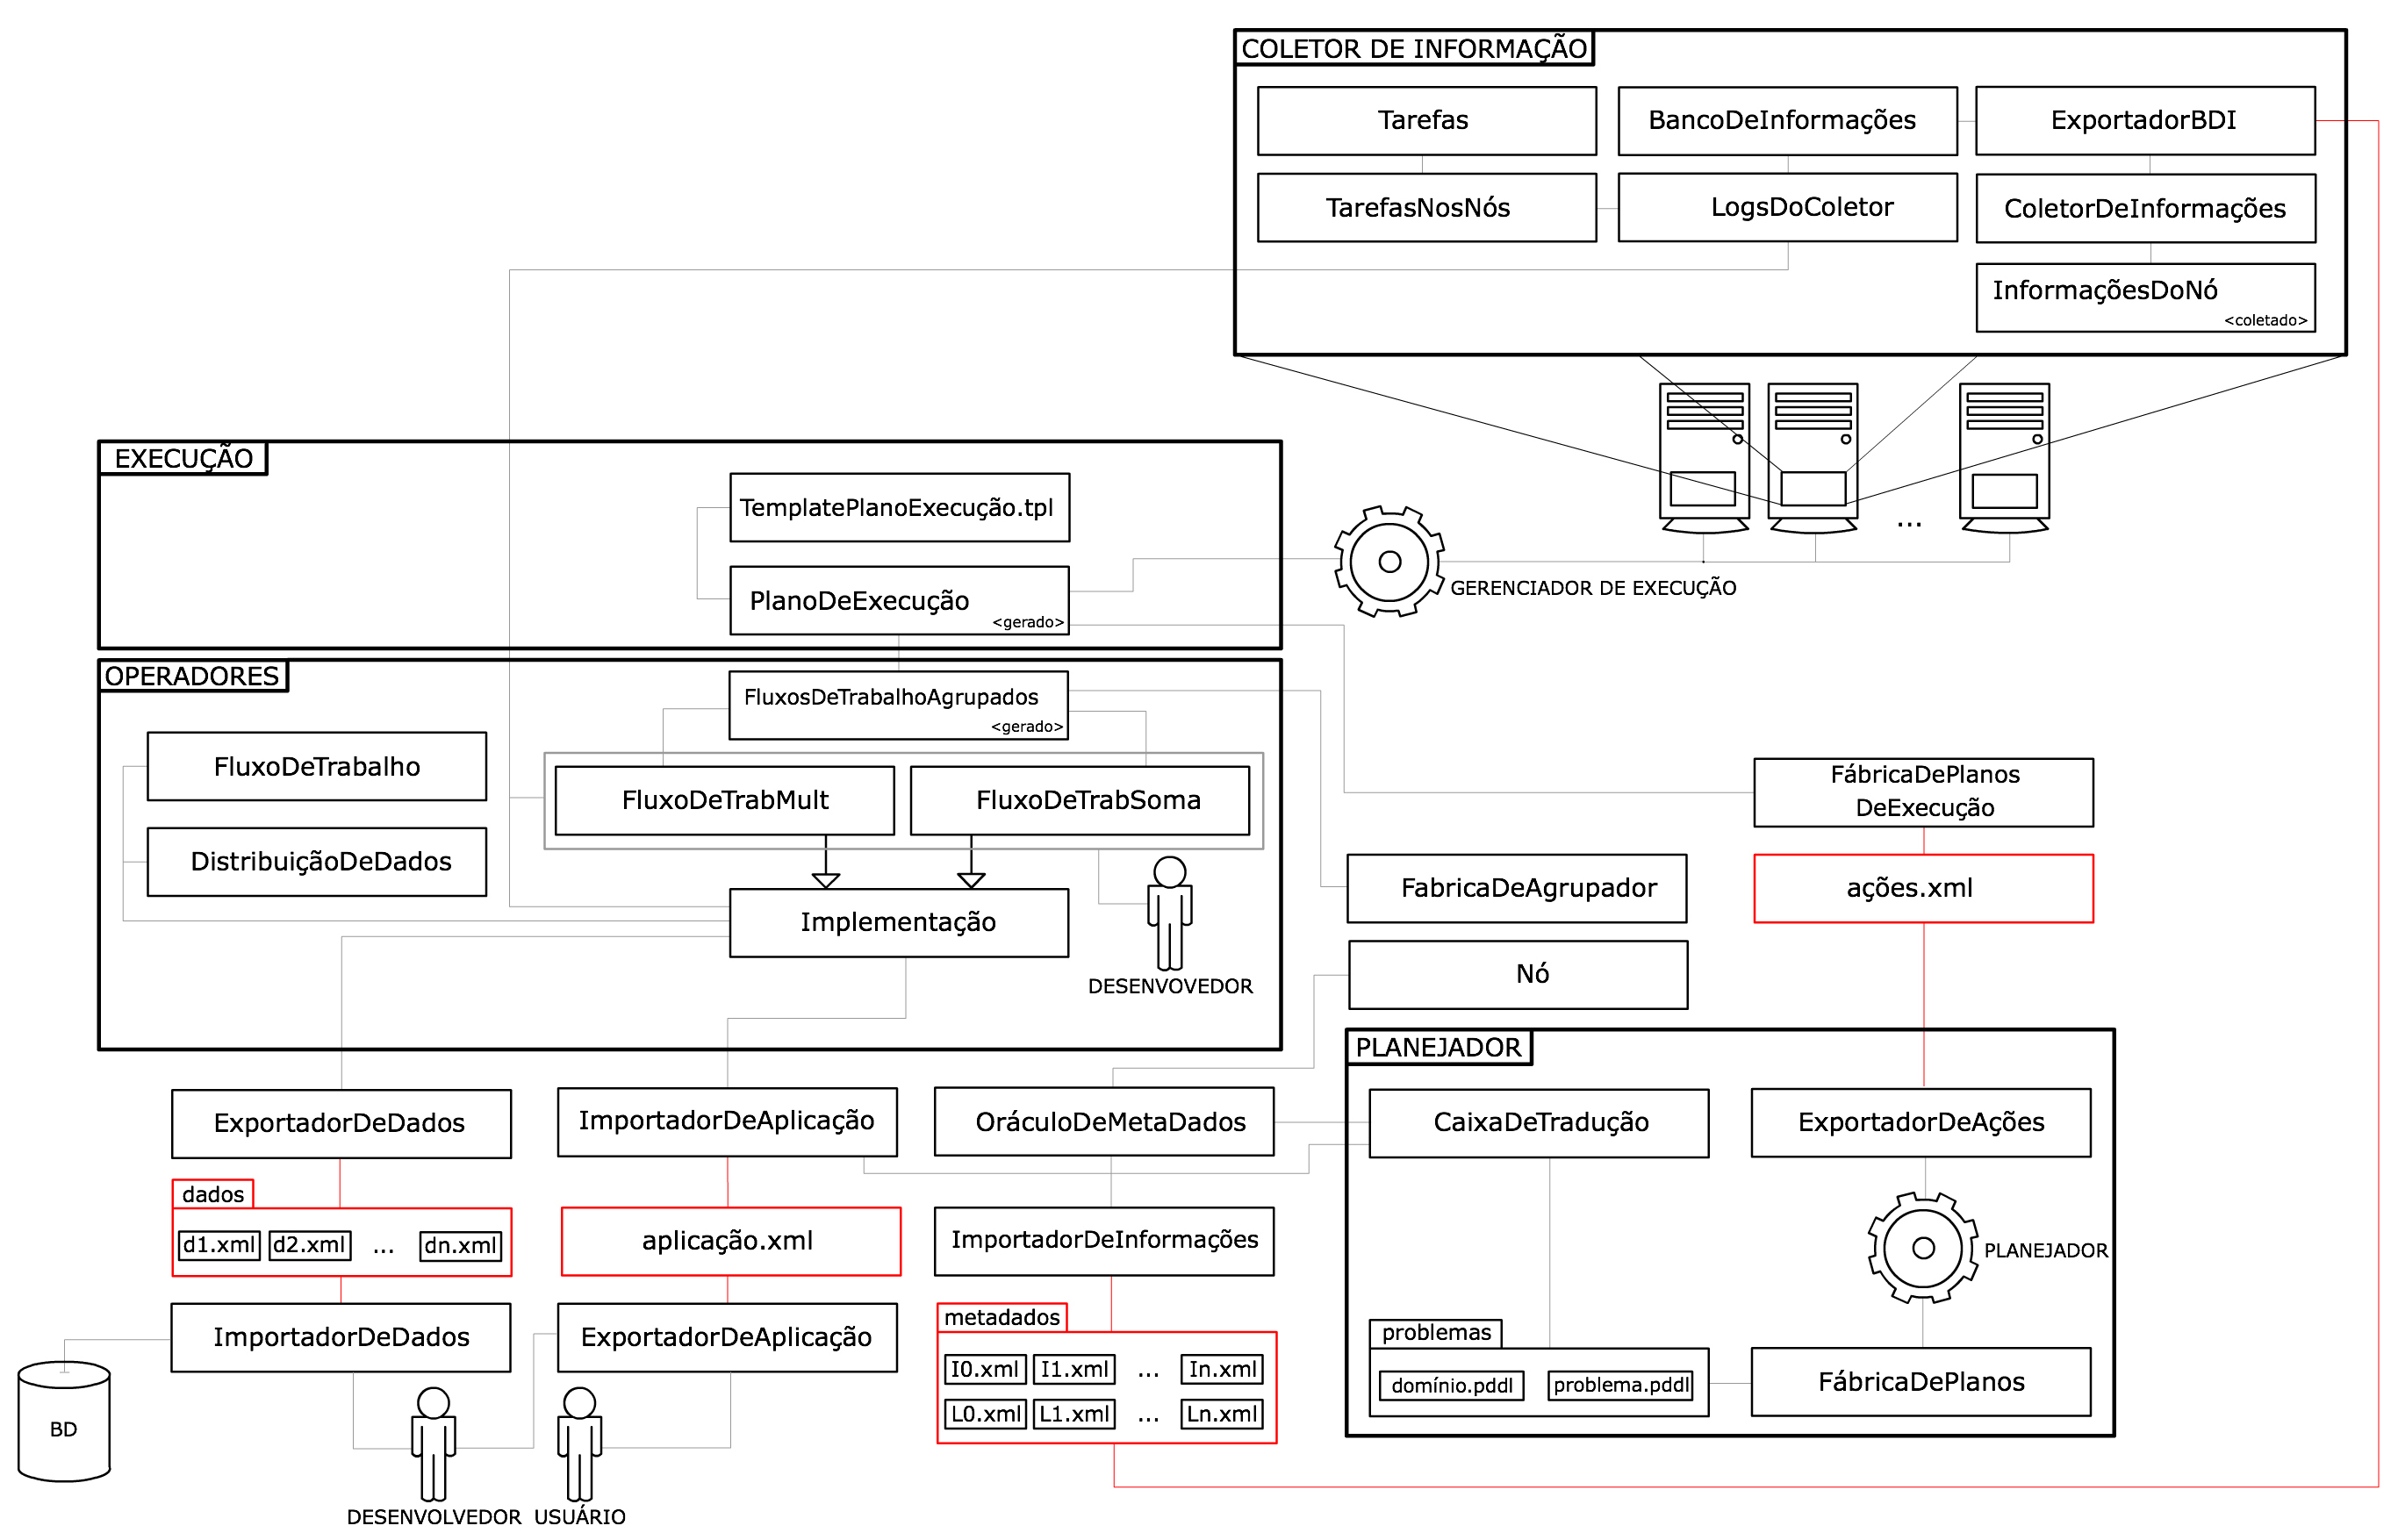
\includegraphics[width=12.8cm]{../images/fig_sys_detailed_red.jpg}
	\end{changemargin}
\end{frame}


\begin{frame}
    \frametitle{Paralelismos}
    \begin{itemize}
		\item paralelismo sobre dados:
		\begin{itemize}
			\item divis�o do processamento de um �nico fluxo de trabalho;
			\item desenvolvedor insere as configura��es (n�mero de n�s ou tamanho dos blocos);
		\end{itemize}
		\item paralelismo sobre execu��o:
		\begin{itemize}
			\item paralelismo entre execu��o de m�ltiplos fluxos de trabalho;
			\item plano paralelo: pondera as depend�ncias de dados;
			\item ordem correta de execu��o;
		\end{itemize}
	\end{itemize}
\end{frame}

\begin{frame}
    \frametitle{Exemplos de Paralelismo - Plano de Execu��o}
	\begin{center}
	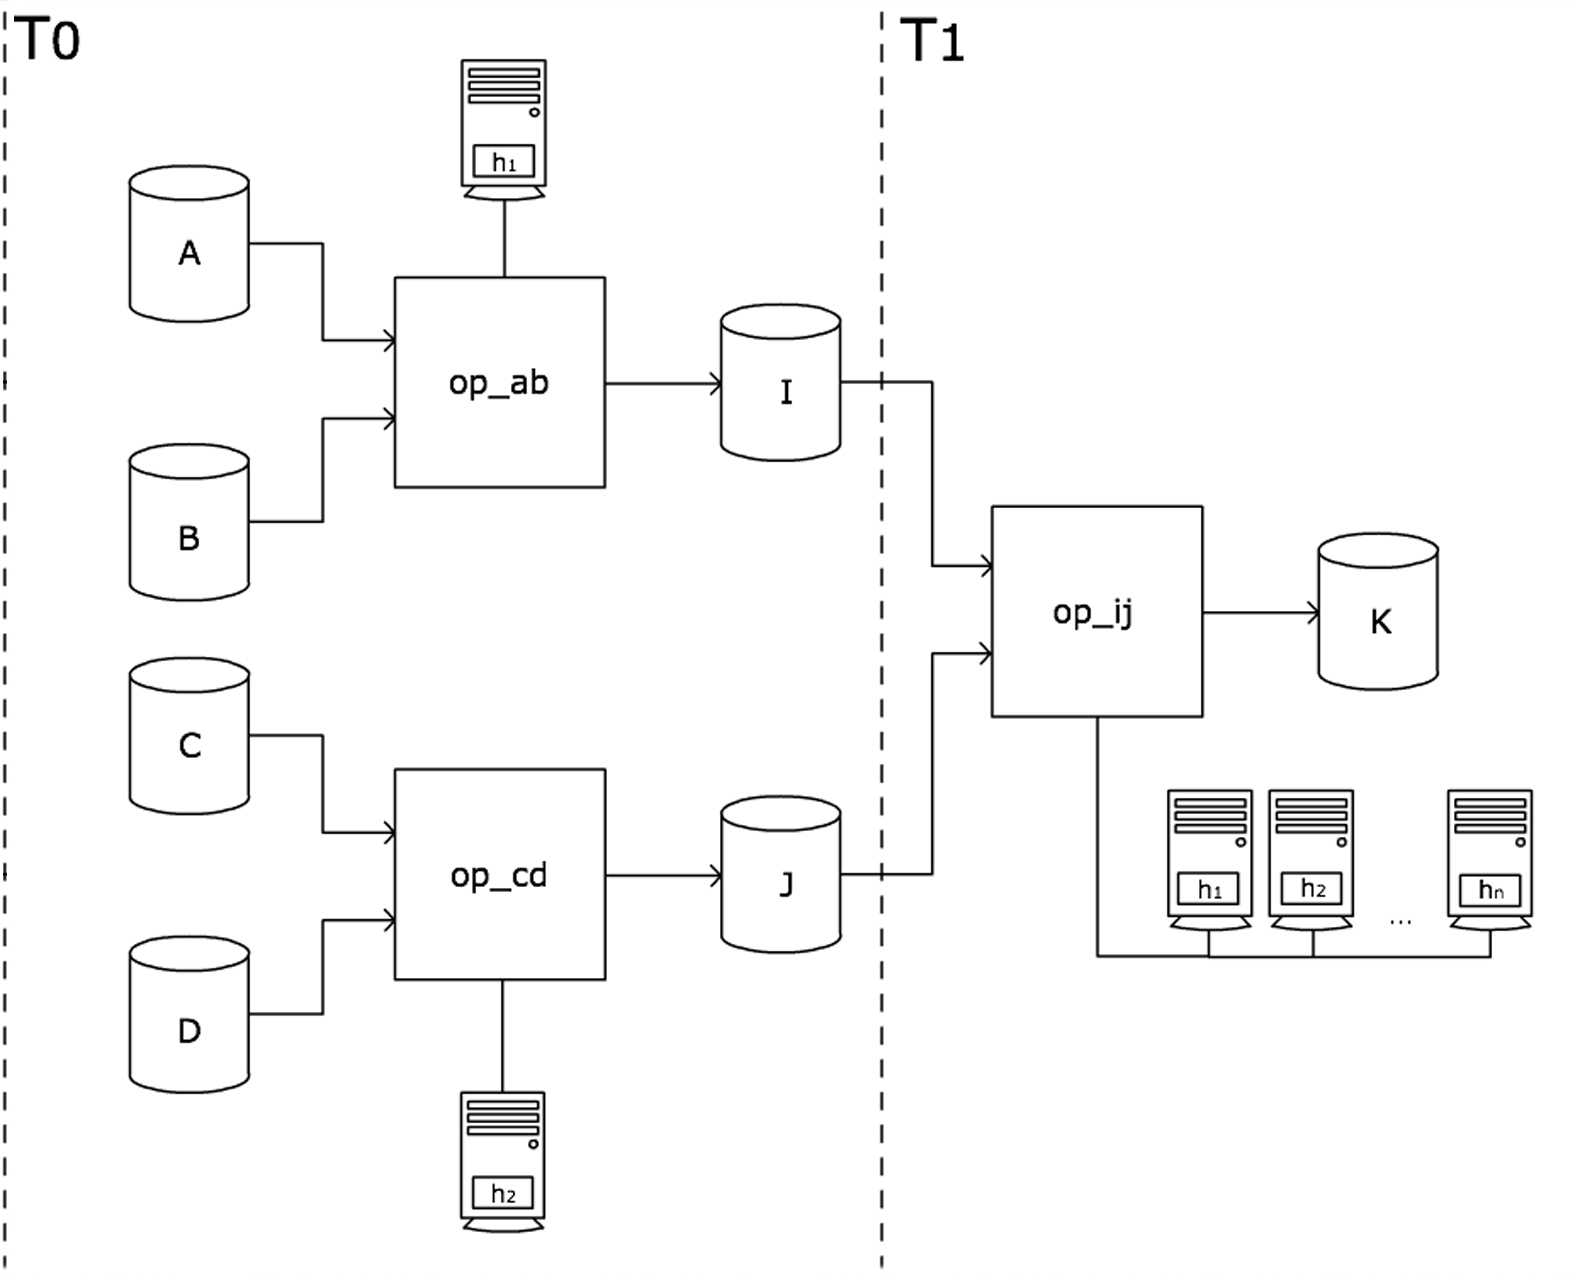
\includegraphics[width=9cm]{../images/fig_sys_parallel_model.jpg}
	\end{center}
\end{frame}

\begin{frame}
    \frametitle{M�trica Flex�vel}
    \begin{itemize}
		\item planejamento baseado nos custos das a��es;
		\item or�culo:
		\begin{itemize}
			\item verifica-se a taxa de ocupa��o dos n�s (livre, parcialmente ocupado ou ocupado);
			\item aplica-se custos pr�-definidos para cada uma das situa��es;
		\end{itemize}
		\item utiliza��o do planejamento de custos para aplica��o de outras m�tricas:
		\begin{itemize}
			\item minimiza��o do consumo de energia el�trica;
			\item maximiza��o de aproveitamento dos recursos;
		\end{itemize}
		\item quantidade de trabalho pode variar de acordo com a situa��o dos recursos, em planos diferentes;
	\end{itemize}
\end{frame}
\chapter{Experimentos}
\label{experimentos}

Neste cap�tulo apresentam-se os experimentos realizados no sistema desenvolvido. A se��o \ref{ex1} mostra um experimento que demonstra a t�cnica de paraleliza��o direta. Na se��o \ref{ex2} apresenta-se um experimento para avalia��o do comportamento utilizando v�rios encadeamentos no fluxo de trabalho. Na se��o \ref{ex3} apresenta-se uma abordagem que demonstra a implementa��o de um operador que trabalha com m�ltiplas entradas e sa�das. Na se��o \ref{ex-consideracoes} faz-se uma analise dos resultados obtidos.

\vspace{1.5cm}

O principal objetivo na an�lise dos resultados est� na corretude dos experimentos bem como a qualidade dos planos gerados. Para os experimentos \ref{ex1} e \ref{ex3} utilizou-se um ambiente de execu��o local no qual simulou-se um ambiente distribu�do. Desta forma, possibilitou-se a reprodu��o dos experimentos com n�s emulados na mesma m�quina. O experimento \ref{ex2} foi um teste para a valida��o do modelo, executado em um ambiente distribu�do com 4 n�s.

A m�quina utilizada para execu��o local possui um processador 2.66 GHz Intel Core 2 Duo com 4GB de mem�ria. As m�quinas do ambiente distribu�do possuem um AMD Opteron com 2.4 GHz e 2GB de mem�ria.

Os testes utilizaram como base os dados extra�dos de matrizes. A motiva��o para a utiliza��o de matrizes � a necessidade de c�lculos simples sobre um grande volume de dados cient�ficos. Para a valida��o do experimento foram utilizadas matrizes quadradas preenchidas por n�meros aleat�rios. Dois operadores foram implementados: soma e multiplica��o de matrizes.

Nas figuras dispostas nesse cap�tulo, cada quadrado representa um operador. Cada operador possui uma identifica��o dos dados que s�o trabalhados. Por exemplo, \emph{op\_a\_b} significa que o operador est� trabalhando com os dados $A$ e $B$. Dentro do quadrado, descreve-se ainda uma informa��o que mostra qual a opera��o efetuada com os dados em quest�o. Por exemplo, \emph{SUM} para soma ou \emph{MULT} para multiplica��o. Os dados s�o representados por cilindros, cada conjunto de dados representa uma matriz e sua identifica��o se d� por letras em mai�sculo. As setas indicam o fluxo dos dados.

Nas tabelas est�o apresentados os resumos de execu��o dos fluxos de trabalho, bem como o plano gerado pelo planejador. A coluna ordem, define a sequencia de execu��o de uma a��o no plano de execu��o. Se uma mesma ordem � repetida em mais de um linha, significa que as a��es ocorrerem em paralelo. A coluna n�, indica qual o n� selecionado para a execu��o da a��o. Se a c�lula apresenta o caractere $*$, significa que a a��o foi executada por todos os n�s. 

Ainda � poss�vel que um subconjunto espec�fico de n�s execute uma a��o, nesse caso suas identifica��es est�o separadas por v�rgula. A coluna operador indica qual o operador utilizado. Se o operador � identificado como \emph{difundir} ent�o h� uma barreira para a publica��o das informa��es, geradas at� o momento, para todos os outros n�s. A coluna dados, indica os dados utilizados para a aplica��o do operador. Quando um dado est� na mesma linha que possui um operador difundir, esse dado � o que ser� publicado para todo o conjunto de n�s. A coluna tempo indica o tempo de execu��o de cada uma das a��es em \UFPRsigla{ms}. As �ltimas linhas mostram um resumo do tempo de execu��o de cada etapa: planejamento, tradu��o, difus�o e processamento. A �ltima linha mostra o tempo total de execu��o.

\section{Experimento 1 - Paraleliza��o Direta}
\label{ex1}

A representa��o do esquema de execu��o dos fluxos de trabalho est�o dispostos na figura \ref{fig:ex1}.

\begin{figure}[ht]
    \centering
    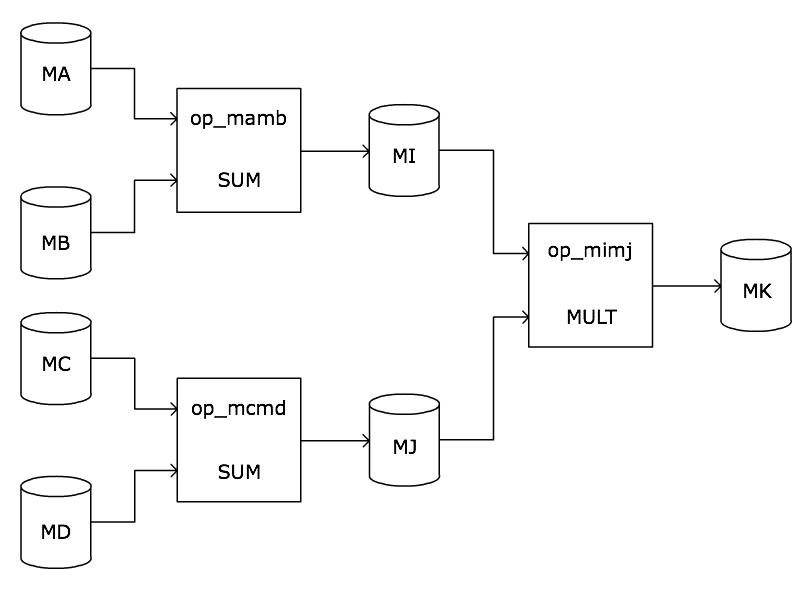
\includegraphics[width=11cm]{images/fig_ex1.jpg}
    \caption{Experimento com opera��es entre matrizes}
    \label{fig:ex1}
\end{figure}

No exemplo s�o definidas tr�s operadores: $op_{\{ma,mb\}}$, $op_{\{mc,md\}}$ e $op_{\{mi,mj\}}$. O operador $op_{\{ma,mb\}}$ espera como entrada os dados $MA$ e $MB$ e gera como sa�da $MI$. J� $op_{\{mc,md\}}$ espera como entrada $MC$ e $MD$ e gera como sa�da $MJ$. O operador $op_{\{mi,mj\}}$ espera como entrada $MI$ e $MJ$ e gera como sa�da $MK$, que em nosso exemplo � o objetivo. A defini��o do arquivo que cont�m a descri��o dos fluxos de trabalho est� transcrita no ap�ndice \ref{ap-aplicacao}.

Foram utilizados dois n�s para a execu��o do experimento: $h_0$ e $h_1$. Neste experimento, analisa-se os modelos paralelos abordados no cap�tulo \ref{modelo}. A \emph{paraleliza��o direta} (se��o \ref{par-direta}) e o \emph{paralelismo sobre execu��o} (se��o \ref{paralelismo-execucao}). A figura \ref{fig:ex1_parallel} mostra a distribui��o das tarefas e os respectivos n�s utilizados para execu��o.

\begin{figure}[ht]
    \centering
    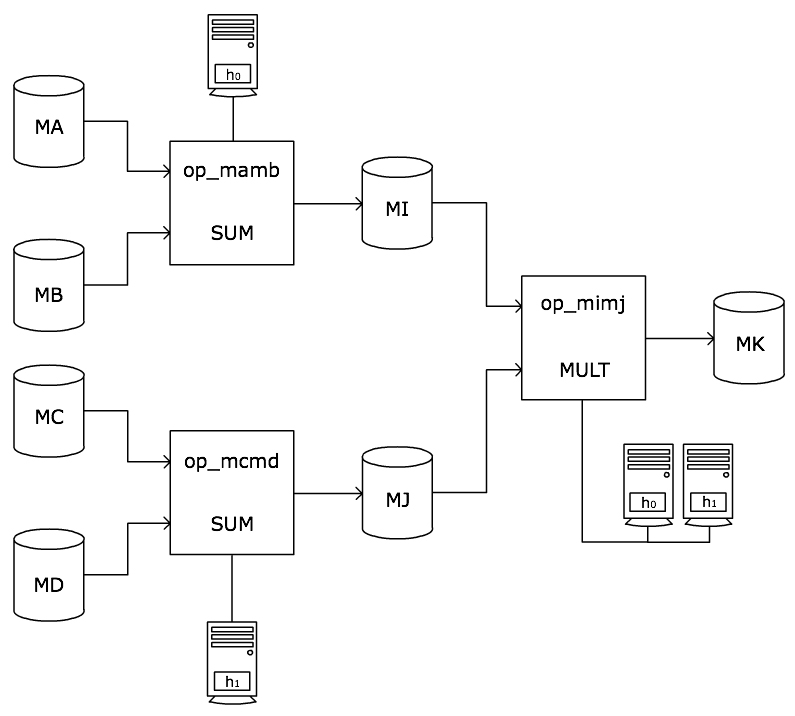
\includegraphics[width=11cm]{images/fig_ex1_parallel.jpg}
    \caption{Diagrama do experimento 1}
    \label{fig:ex1_parallel}
\end{figure}

A paraleliza��o direta ocorre na execu��o distribu�da do operador $op_{\{mi,mj\}}$. O paralelismo sobre execu��o est� exemplificado na execu��o simult�nea de $op_{\{ma,mb\}}$ e $op_{\{mc,md\}}$.

A tabela \ref{tab:ex1} detalha as informa��es extra�das do experimento.

\begin{table}[ht]
	\centering
	\caption{Resultados do experimento com paraleliza��o direta}
	\label{tab:ex1}
	\begin{tabular}{|l|l|l|l|l|}
	\hline
	\multicolumn{1}{|c|}{Ordem} & \multicolumn{1}{c|}{Host} & \multicolumn{1}{c|}{Operador} & \multicolumn{1}{c|}{Dados} & \multicolumn{1}{c|}{Tempo (ms)} \\ 
	\hline
	\multicolumn{1}{|c|}{1} & \multicolumn{1}{c|}{$h_0$} & \multicolumn{1}{c|}{SUM} & \multicolumn{1}{c|}{$MA,MB$} & \multicolumn{1}{r|}{4779} \\ 
	\hline
	\multicolumn{1}{|c|}{1} & \multicolumn{1}{c|}{$h_1$} & \multicolumn{1}{c|}{SUM} & \multicolumn{1}{c|}{$MC,MD$} & \multicolumn{1}{r|}{3935} \\ 
	\hline
	\multicolumn{1}{|c|}{2} & \multicolumn{1}{c|}{*} & \multicolumn{1}{c|}{DIFUNDIR} & \multicolumn{1}{c|}{$MI$} & \multicolumn{1}{r|}{5617} \\ 
	\hline
	\multicolumn{1}{|c|}{2} & \multicolumn{1}{c|}{*} & \multicolumn{1}{c|}{DIFUNDIR} & \multicolumn{1}{c|}{$MJ$} & \multicolumn{1}{r|}{4203} \\ 
	\hline
	\multicolumn{1}{|c|}{3} & \multicolumn{1}{c|}{$h_0, h_1$} & \multicolumn{1}{c|}{MULT} & \multicolumn{1}{c|}{$MI,MJ$} & \multicolumn{1}{r|}{3170} \\ 
	\hline
	\multicolumn{1}{|c|}{4} & \multicolumn{1}{c|}{*} & \multicolumn{1}{c|}{DIFUNDIR} & \multicolumn{1}{c|}{$MK$} & \multicolumn{1}{r|}{2880} \\ 
	\hline
	\multicolumn{1}{|c|}{5} & \multicolumn{1}{c|}{*} & \multicolumn{1}{c|}{coletor de informa��o} & \multicolumn{1}{c|}{metadados} & \multicolumn{1}{r|}{31} \\ 
	\hline
	\multicolumn{4}{|c|}{tempo de planejamento} & \multicolumn{1}{r|}{1014} \\ 
	\hline
	\multicolumn{4}{|c|}{tempo de tradu��o} & \multicolumn{1}{r|}{523} \\ 
	\hline
	\multicolumn{4}{|c|}{tempo de difus�o} & \multicolumn{1}{r|}{12700} \\ 
	\hline
	\multicolumn{4}{|c|}{tempo processamento} & \multicolumn{1}{r|}{11935} \\ 
	\hline
	\multicolumn{4}{|c|}{tempo total} & \multicolumn{1}{r|}{26172} \\ 
	\hline
	\end{tabular}
\end{table}

Nota-se que o planejador considerou a execu��o simult�nea dos operadores $op_{\{ma,mb\}}$ e $op_{\{mc,md\}}$ na etapa $1$, pois os operadores n�o possuem qualquer depend�ncia de dados. O tempo para execu��o da opera��o de soma foi semelhante, para o operador $op_{\{ma,mb\}}$ gastou-se $4779$ms, enquanto que o operador $op_{\{mc,md\}}$ terminou a execu��o em $3935$ms. 

Nas etapas $2$ e $4$ nota-se a opera��o de difus�o. Essa opera��o distribui os resultados obtidos pelos operadores para todos os outros n�s do ambiente, visto que algum operador seguinte pode utilizar os dados gerados na opera��o em quest�o.

A etapa $3$ utiliza dois n�s para a execu��o da opera��o de multiplica��o. O tipo de paraleliza��o adotada � direta, por isso, o desenvolvedor informa os par�metros para a execu��o paralela dos dados. Ambos os n�s dispon�veis foram escolhidos para a divis�o dos dados, e a opera��o completa levou $3170$ms.

\section{Experimento 2 - Encadeamento de Fluxos de Trabalho}
\label{ex2}

A representa��o do esquema de execu��o do fluxo de trabalho est� disposta na figura \ref{fig:ex2}.

\begin{landscape}
	
\begin{figure}[ht]
    \centering
    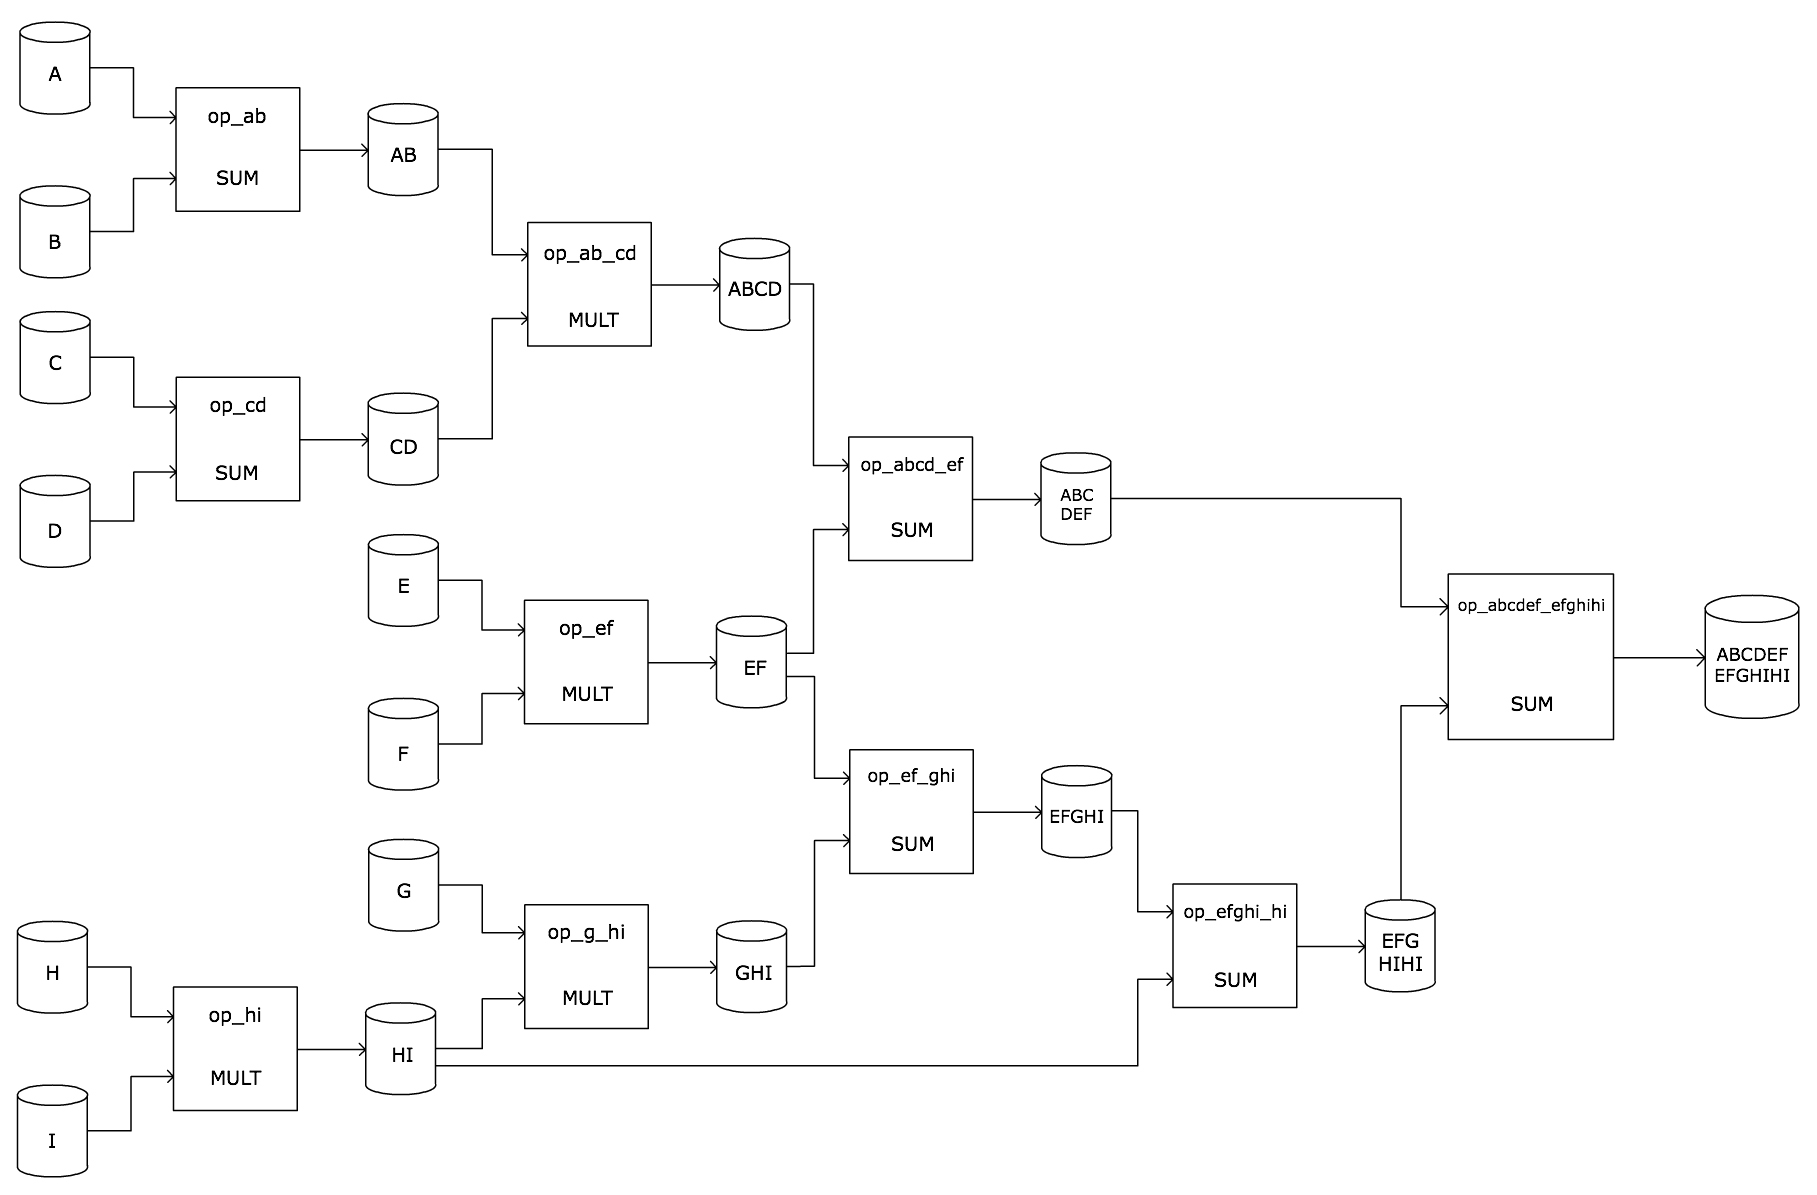
\includegraphics[width=22cm]{images/fig_ex2.jpg}
    \caption{Diagrama do experimento 2}
    \label{fig:ex2}
\end{figure}

\end{landscape}

No exemplo s�o definidos dez operadores: $op_{\{a,b\}}$, $op_{\{c,d\}}$, $op_{\{h,i\}}$, $ op_{\{e,f\}}$, $op_{\{ab,cd\}}$, $op_{\{g,hi\}}$, $op_{\{abcd,ef\}}$, $op_{\{ef,ghi\}}$, $op_{\{efghi_hi\}}$ e $op_{\{abcdef,efghihi\}}$. A indexa��o de cada operador define sua entrada de dados. O objetivo do experimento � a obten��o do dado final $ABCDEFEFGHIHI$.

Para o experimento foram utilizados 4 n�s: $h_0, h_1, h_2$ e $h_3$. Testou-se a validade do componente \emph{Or�culoDeMetaDados} que retorna a taxa de ocupa��o dos n�s dispon�veis, em tr�s situa��es diferentes:

\begin{enumerate}
	\item quatro n�s dispon�veis;
	\item dois n�s dispon�veis ($h_0$ e $h_1$) e dois n�s parcialmente dispon�veis ($h_2$ e $h_3$);
	\item um n� dispon�vel ($h_0$) e tr�s parcialmente dispon�veis ($h_1$, $h_2$ e $h_3$).
\end{enumerate}

As tabelas \ref{tab:ex2a}, \ref{tab:ex2b}, \ref{tab:ex2c} demonstram os resultados para as tr�s situa��es, respectivamente.

\newpage

\begin{table}[ht]
	\centering
	\caption{Encadeamento de fluxos - 4 n�s dispon�veis}
	\label{tab:ex2a}
	\begin{tabular}{|l|l|l|l|l|}
	\hline
	\multicolumn{1}{|c|}{Ordem} & \multicolumn{1}{c|}{Host} & \multicolumn{1}{c|}{Operador} & \multicolumn{1}{c|}{Dados} & \multicolumn{1}{c|}{Tempo (ms)} \\ 
	\hline
	\multicolumn{1}{|c|}{1} & \multicolumn{1}{c|}{$h_1$} & \multicolumn{1}{c|}{MULT} & \multicolumn{1}{c|}{$H,I$} & \multicolumn{1}{r|}{17400} \\ 
	\hline
	\multicolumn{1}{|c|}{1} & \multicolumn{1}{c|}{$h_3$} & \multicolumn{1}{c|}{MULT} & \multicolumn{1}{c|}{$E,F$} & \multicolumn{1}{r|}{17160} \\ 
	\hline
	\multicolumn{1}{|c|}{1} & \multicolumn{1}{c|}{$h_0$} & \multicolumn{1}{c|}{SUM} & \multicolumn{1}{c|}{$C,D$} & \multicolumn{1}{r|}{16699} \\ 
	\hline
	\multicolumn{1}{|c|}{1} & \multicolumn{1}{c|}{$h_2$} & \multicolumn{1}{c|}{SUM} & \multicolumn{1}{c|}{$A,B$} & \multicolumn{1}{r|}{17738} \\ 
	\hline
	\multicolumn{1}{|c|}{2} & \multicolumn{1}{c|}{*} & \multicolumn{1}{c|}{DIFUNDIR} & \multicolumn{1}{c|}{$EF$} & \multicolumn{1}{r|}{16616} \\ 
	\hline
	\multicolumn{1}{|c|}{2} & \multicolumn{1}{c|}{*} & \multicolumn{1}{c|}{DIFUNDIR} & \multicolumn{1}{c|}{$HI$} & \multicolumn{1}{r|}{15818} \\ 
	\hline
	\multicolumn{1}{|c|}{2} & \multicolumn{1}{c|}{*} & \multicolumn{1}{c|}{DIFUNDIR} & \multicolumn{1}{c|}{$AB$} & \multicolumn{1}{r|}{14650} \\ 
	\hline
	\multicolumn{1}{|c|}{2} & \multicolumn{1}{c|}{*} & \multicolumn{1}{c|}{DIFUNDIR} & \multicolumn{1}{c|}{$CD$} & \multicolumn{1}{r|}{14472} \\ 
	\hline
	\multicolumn{1}{|c|}{3} & \multicolumn{1}{c|}{$h_2$} & \multicolumn{1}{c|}{MULT} & \multicolumn{1}{c|}{$G,HI$} & \multicolumn{1}{r|}{13168} \\ 
	\hline
	\multicolumn{1}{|c|}{3} & \multicolumn{1}{c|}{$h_0$} & \multicolumn{1}{c|}{MULT} & \multicolumn{1}{c|}{$AB,CD$} & \multicolumn{1}{r|}{14475} \\ 
	\hline
	\multicolumn{1}{|c|}{4} & \multicolumn{1}{c|}{*} & \multicolumn{1}{c|}{DIFUNDIR} & \multicolumn{1}{c|}{$GHI$} & \multicolumn{1}{r|}{14908} \\ 
	\hline
	\multicolumn{1}{|c|}{4} & \multicolumn{1}{c|}{*} & \multicolumn{1}{c|}{DIFUNDIR} & \multicolumn{1}{c|}{$ABCD$} & \multicolumn{1}{r|}{14637} \\ 
	\hline
	\multicolumn{1}{|c|}{5} & \multicolumn{1}{c|}{$h_1$} & \multicolumn{1}{c|}{SUM} & \multicolumn{1}{c|}{$EF,GHI$} & \multicolumn{1}{r|}{14189} \\ 
	\hline
	\multicolumn{1}{|c|}{5} & \multicolumn{1}{c|}{$h_3$} & \multicolumn{1}{c|}{SUM} & \multicolumn{1}{c|}{$ABCD,EF$} & \multicolumn{1}{r|}{13622} \\ 
	\hline
	\multicolumn{1}{|c|}{6} & \multicolumn{1}{c|}{*} & \multicolumn{1}{c|}{DIFUNDIR} & \multicolumn{1}{c|}{$EFGHI$} & \multicolumn{1}{r|}{14661} \\ 
	\hline
	\multicolumn{1}{|c|}{6} & \multicolumn{1}{c|}{*} & \multicolumn{1}{c|}{DIFUNDIR} & \multicolumn{1}{c|}{$ABCDEF$} & \multicolumn{1}{r|}{14881} \\ 
	\hline
	\multicolumn{1}{|c|}{7} & \multicolumn{1}{c|}{$h_3$} & \multicolumn{1}{c|}{SUM} & \multicolumn{1}{c|}{$EFGHI,HI$} & \multicolumn{1}{r|}{13584} \\ 
	\hline
	\multicolumn{1}{|c|}{8} & \multicolumn{1}{c|}{*} & \multicolumn{1}{c|}{DIFUNDIR} & \multicolumn{1}{c|}{$EFGHIHI$} & \multicolumn{1}{r|}{15042} \\ 
	\hline
	\multicolumn{1}{|c|}{9} & \multicolumn{1}{c|}{$h_0$} & \multicolumn{1}{c|}{SUM} & \multicolumn{1}{c|}{$ABCDEF,EFGHIHI$} & \multicolumn{1}{r|}{14900} \\ 
	\hline
	\multicolumn{1}{|c|}{10} & \multicolumn{1}{c|}{*} & \multicolumn{1}{c|}{DIFUNDIR} & \multicolumn{1}{c|}{$ABCDEFEFGHIHI$} & \multicolumn{1}{r|}{15145} \\ 
	\hline
	\multicolumn{1}{|c|}{11} & \multicolumn{1}{c|}{*} & \multicolumn{1}{c|}{coletor de informa��o} & \multicolumn{1}{c|}{metadados} & \multicolumn{1}{r|}{39} \\ 
	\hline
	\multicolumn{4}{|c|}{tempo de planejamento} & \multicolumn{1}{r|}{3523} \\ 
	\hline
	\multicolumn{4}{|c|}{tempo de tradu��o} & \multicolumn{1}{r|}{1301} \\ 
	\hline
	\multicolumn{4}{|c|}{tempo de difus�o} & \multicolumn{1}{r|}{150830} \\ 
	\hline
	\multicolumn{4}{|c|}{tempo processamento} & \multicolumn{1}{r|}{153016} \\ 
	\hline
	\multicolumn{4}{|c|}{tempo total} & \multicolumn{1}{r|}{308670} \\ 
	\hline
	\end{tabular}
\end{table}

Nota-se que com 4 n�s dispon�veis o planejador elabora o plano �timo, distribuindo o m�ximo de operadores poss�vel na etapa $1$. A difus�o dos resultados ocorre nas etapas $2$, $4$, $6$, $8$ e $10$. As etapas �mpares s�o respons�veis pelos c�lculos dos operadores enquanto que as etapas pares s�o respons�veis pela difus�o dos resultados obtidos.

\newpage

\begin{table}[ht]
	\centering
	\caption{Encadeamento de fluxos - 2 n�s dispon�veis e 2 parcialmente dispon�veis}
	\label{tab:ex2b}
	\begin{tabular}{|l|l|l|l|l|}
	\hline
	\multicolumn{1}{|c|}{Ordem} & \multicolumn{1}{c|}{Host} & \multicolumn{1}{c|}{Operador} & \multicolumn{1}{c|}{Dados} & \multicolumn{1}{c|}{Tempo (ms)} \\ 
	\hline
	\multicolumn{1}{|c|}{1} & \multicolumn{1}{c|}{$h_1$} & \multicolumn{1}{c|}{MULT} & \multicolumn{1}{c|}{$H,I$} & \multicolumn{1}{r|}{18999} \\ 
	\hline
	\multicolumn{1}{|c|}{1} & \multicolumn{1}{c|}{$h_0$} & \multicolumn{1}{c|}{SUM} & \multicolumn{1}{c|}{$C,D$} & \multicolumn{1}{r|}{17012} \\ 
	\hline
	\multicolumn{1}{|c|}{1} & \multicolumn{1}{c|}{$h_3$} & \multicolumn{1}{c|}{SUM} & \multicolumn{1}{c|}{$A,B$} & \multicolumn{1}{r|}{17541} \\ 
	\hline
	\multicolumn{1}{|c|}{2} & \multicolumn{1}{c|}{*} & \multicolumn{1}{c|}{DIFUNDIR} & \multicolumn{1}{c|}{$HI$} & \multicolumn{1}{r|}{17243} \\ 
	\hline
	\multicolumn{1}{|c|}{2} & \multicolumn{1}{c|}{*} & \multicolumn{1}{c|}{DIFUNDIR} & \multicolumn{1}{c|}{$CD$} & \multicolumn{1}{r|}{16543} \\ 
	\hline
	\multicolumn{1}{|c|}{2} & \multicolumn{1}{c|}{*} & \multicolumn{1}{c|}{DIFUNDIR} & \multicolumn{1}{c|}{$AB$} & \multicolumn{1}{r|}{15426} \\ 
	\hline
	\multicolumn{1}{|c|}{3} & \multicolumn{1}{c|}{$h_1$} & \multicolumn{1}{c|}{MULT} & \multicolumn{1}{c|}{$E,F$} & \multicolumn{1}{r|}{15188} \\ 
	\hline
	\multicolumn{1}{|c|}{3} & \multicolumn{1}{c|}{$h_0$} & \multicolumn{1}{c|}{MULT} & \multicolumn{1}{c|}{$G,HI$} & \multicolumn{1}{r|}{13453} \\ 
	\hline
	\multicolumn{1}{|c|}{4} & \multicolumn{1}{c|}{*} & \multicolumn{1}{c|}{DIFUNDIR} & \multicolumn{1}{c|}{$EF$} & \multicolumn{1}{r|}{15377} \\ 
	\hline
	\multicolumn{1}{|c|}{4} & \multicolumn{1}{c|}{*} & \multicolumn{1}{c|}{DIFUNDIR} & \multicolumn{1}{c|}{$GHI$} & \multicolumn{1}{r|}{15170} \\ 
	\hline
	\multicolumn{1}{|c|}{5} & \multicolumn{1}{c|}{$h_1$} & \multicolumn{1}{c|}{SUM} & \multicolumn{1}{c|}{$EF,GHI$} & \multicolumn{1}{r|}{15286} \\ 
	\hline
	\multicolumn{1}{|c|}{5} & \multicolumn{1}{c|}{$h_0$} & \multicolumn{1}{c|}{MULT} & \multicolumn{1}{c|}{$AB,CD$} & \multicolumn{1}{r|}{14212} \\ 
	\hline
	\multicolumn{1}{|c|}{6} & \multicolumn{1}{c|}{*} & \multicolumn{1}{c|}{DIFUNDIR} & \multicolumn{1}{c|}{$EFGHI$} & \multicolumn{1}{r|}{15334} \\ 
	\hline
	\multicolumn{1}{|c|}{6} & \multicolumn{1}{c|}{*} & \multicolumn{1}{c|}{DIFUNDIR} & \multicolumn{1}{c|}{$ABCD$} & \multicolumn{1}{r|}{15415} \\ 
	\hline
	\multicolumn{1}{|c|}{7} & \multicolumn{1}{c|}{$h_2$} & \multicolumn{1}{c|}{SUM} & \multicolumn{1}{c|}{$EFGHI,HI$} & \multicolumn{1}{r|}{13484} \\ 
	\hline
	\multicolumn{1}{|c|}{7} & \multicolumn{1}{c|}{$h_3$} & \multicolumn{1}{c|}{SUM} & \multicolumn{1}{c|}{$ABCD, EF$} & \multicolumn{1}{r|}{13389} \\ 
	\hline
	\multicolumn{1}{|c|}{8} & \multicolumn{1}{c|}{*} & \multicolumn{1}{c|}{DIFUNDIR} & \multicolumn{1}{c|}{$EFGHIHI$} & \multicolumn{1}{r|}{15433} \\ 
	\hline
	\multicolumn{1}{|c|}{8} & \multicolumn{1}{c|}{*} & \multicolumn{1}{c|}{DIFUNDIR} & \multicolumn{1}{c|}{$ABCDEF$} & \multicolumn{1}{r|}{15423} \\ 
	\hline
	\multicolumn{1}{|c|}{9} & \multicolumn{1}{c|}{$h_3$} & \multicolumn{1}{c|}{SUM} & \multicolumn{1}{c|}{$ABCDEF,EFGHIHI$} & \multicolumn{1}{r|}{13634} \\ 
	\hline
	\multicolumn{1}{|c|}{10} & \multicolumn{1}{c|}{*} & \multicolumn{1}{c|}{DIFUNDIR} & \multicolumn{1}{c|}{$ABCDEFEFGHIHI$} & \multicolumn{1}{r|}{15518} \\ 
	\hline
	\multicolumn{1}{|c|}{11} & \multicolumn{1}{c|}{*} & \multicolumn{1}{c|}{coletor de informa��o} & \multicolumn{1}{c|}{metadados} & \multicolumn{1}{r|}{10} \\ 
	\hline
	\multicolumn{4}{|c|}{tempo de planejamento} & \multicolumn{1}{r|}{2285} \\ 
	\hline
	\multicolumn{4}{|c|}{tempo de tradu��o} & \multicolumn{1}{r|}{1043} \\ 
	\hline
	\multicolumn{4}{|c|}{tempo de difus�o} & \multicolumn{1}{r|}{156882} \\ 
	\hline
	\multicolumn{4}{|c|}{tempo processamento} & \multicolumn{1}{r|}{152279} \\ 
	\hline
	\multicolumn{4}{|c|}{tempo total} & \multicolumn{1}{r|}{312489} \\ 
	\hline
	\end{tabular}
\end{table}

Ao trabalhar com dois n�s parcialmente dispon�veis, o planejador optou por um plano no qual em um primeiro momento apenas 3 n�s s�o utilizados. Entretanto gerou-se ainda assim um plano com $10$ etapas. A grande diferen�a � que a etapa $7$ executa paralelamente o operador $op_{\{efghi_hi\}}$ e $op_{\{abcd,ef\}}$. No plano anterior, com todos os n�s dispon�veis, o operador $op_{\{abcd,ef\}}$ � executado na etapa $5$, pois neste momento, todas as depend�ncias j� haviam sido calculadas.

\newpage

\begin{table}[ht]
	\centering
	\caption{Encadeamento de fluxos - 1 n� dispon�vel e 3 parcialmente dispon�veis}
	\label{tab:ex2c}
	\begin{tabular}{|l|l|l|l|l|}
	\hline
	\multicolumn{1}{|c|}{Ordem} & \multicolumn{1}{c|}{Host} & \multicolumn{1}{c|}{Operador} & \multicolumn{1}{c|}{Dados} & \multicolumn{1}{c|}{Tempo (ms)} \\ 
	\hline
	\multicolumn{1}{|c|}{1} & \multicolumn{1}{c|}{$h_0$} & \multicolumn{1}{c|}{MULT} & \multicolumn{1}{c|}{$E,F$} & \multicolumn{1}{r|}{18146} \\ 
	\hline
	\multicolumn{1}{|c|}{1} & \multicolumn{1}{c|}{$h_2$} & \multicolumn{1}{c|}{MULT} & \multicolumn{1}{c|}{$H,I$} & \multicolumn{1}{r|}{17923} \\ 
	\hline
	\multicolumn{1}{|c|}{1} & \multicolumn{1}{c|}{$h_1$} & \multicolumn{1}{c|}{SUM} & \multicolumn{1}{c|}{$C,D$} & \multicolumn{1}{r|}{17075} \\ 
	\hline
	\multicolumn{1}{|c|}{1} & \multicolumn{1}{c|}{$h_3$} & \multicolumn{1}{c|}{SUM} & \multicolumn{1}{c|}{$A,B$} & \multicolumn{1}{r|}{17972} \\ 
	\hline
	\multicolumn{1}{|c|}{2} & \multicolumn{1}{c|}{*} & \multicolumn{1}{c|}{DIFUNDIR} & \multicolumn{1}{c|}{$EF$} & \multicolumn{1}{r|}{16672} \\ 
	\hline
	\multicolumn{1}{|c|}{2} & \multicolumn{1}{c|}{*} & \multicolumn{1}{c|}{DIFUNDIR} & \multicolumn{1}{c|}{$HI$} & \multicolumn{1}{r|}{15897} \\ 
	\hline
	\multicolumn{1}{|c|}{2} & \multicolumn{1}{c|}{*} & \multicolumn{1}{c|}{DIFUNDIR} & \multicolumn{1}{c|}{$AB$} & \multicolumn{1}{r|}{14519} \\ 
	\hline
	\multicolumn{1}{|c|}{2} & \multicolumn{1}{c|}{*} & \multicolumn{1}{c|}{DIFUNDIR} & \multicolumn{1}{c|}{$CD$} & \multicolumn{1}{r|}{14676} \\ 
	\hline
	\multicolumn{1}{|c|}{3} & \multicolumn{1}{c|}{$h_3$} & \multicolumn{1}{c|}{MULT} & \multicolumn{1}{c|}{$G,HI$} & \multicolumn{1}{r|}{13658} \\ 
	\hline
	\multicolumn{1}{|c|}{3} & \multicolumn{1}{c|}{$h_0$} & \multicolumn{1}{c|}{MULT} & \multicolumn{1}{c|}{$AB,CD$} & \multicolumn{1}{r|}{14333} \\ 
	\hline
	\multicolumn{1}{|c|}{4} & \multicolumn{1}{c|}{*} & \multicolumn{1}{c|}{DIFUNDIR} & \multicolumn{1}{c|}{$GHI$} & \multicolumn{1}{r|}{15110} \\ 
	\hline
	\multicolumn{1}{|c|}{4} & \multicolumn{1}{c|}{*} & \multicolumn{1}{c|}{DIFUNDIR} & \multicolumn{1}{c|}{$ABCD$} & \multicolumn{1}{r|}{14909} \\ 
	\hline
	\multicolumn{1}{|c|}{5} & \multicolumn{1}{c|}{$h_3$} & \multicolumn{1}{c|}{SUM} & \multicolumn{1}{c|}{$EF,GHI$} & \multicolumn{1}{r|}{14770} \\ 
	\hline
	\multicolumn{1}{|c|}{5} & \multicolumn{1}{c|}{$h_1$} & \multicolumn{1}{c|}{SUM} & \multicolumn{1}{c|}{$ABCD,EF$} & \multicolumn{1}{r|}{14974} \\ 
	\hline
	\multicolumn{1}{|c|}{6} & \multicolumn{1}{c|}{*} & \multicolumn{1}{c|}{DIFUNDIR} & \multicolumn{1}{c|}{$EFGHI$} & \multicolumn{1}{r|}{14817} \\ 
	\hline
	\multicolumn{1}{|c|}{6} & \multicolumn{1}{c|}{*} & \multicolumn{1}{c|}{DIFUNDIR} & \multicolumn{1}{c|}{$ABCDEF$} & \multicolumn{1}{r|}{15352} \\ 
	\hline
	\multicolumn{1}{|c|}{7} & \multicolumn{1}{c|}{$h_2$} & \multicolumn{1}{c|}{SUM} & \multicolumn{1}{c|}{$EFGHI,HI$} & \multicolumn{1}{r|}{14004} \\ 
	\hline
	\multicolumn{1}{|c|}{8} & \multicolumn{1}{c|}{*} & \multicolumn{1}{c|}{DIFUNDIR} & \multicolumn{1}{c|}{$EFGHIHI$} & \multicolumn{1}{r|}{15235} \\ 
	\hline
	\multicolumn{1}{|c|}{9} & \multicolumn{1}{c|}{$h_2$} & \multicolumn{1}{c|}{SUM} & \multicolumn{1}{c|}{$ABCDEF,EFGHIHI$} & \multicolumn{1}{r|}{14046} \\ 
	\hline
	\multicolumn{1}{|c|}{10} & \multicolumn{1}{c|}{*} & \multicolumn{1}{c|}{DIFUNDIR} & \multicolumn{1}{c|}{$ABCDEFEFGHIHI$} & \multicolumn{1}{r|}{14987} \\ 
	\hline
	\multicolumn{1}{|c|}{11} & \multicolumn{1}{c|}{*} & \multicolumn{1}{c|}{coletor de informa��o} & \multicolumn{1}{c|}{metadados} & \multicolumn{1}{r|}{32} \\ 
	\hline
	\multicolumn{4}{|c|}{tempo de planejamento} & \multicolumn{1}{r|}{2256} \\ 
	\hline
	\multicolumn{4}{|c|}{tempo de tradu��o} & \multicolumn{1}{r|}{1115} \\ 
	\hline
	\multicolumn{4}{|c|}{tempo de difus�o} & \multicolumn{1}{r|}{152174} \\ 
	\hline
	\multicolumn{4}{|c|}{tempo processamento} & \multicolumn{1}{r|}{156973} \\ 
	\hline
	\multicolumn{4}{|c|}{tempo total} & \multicolumn{1}{r|}{312518} \\ 
	\hline
	\end{tabular}
\end{table}

Mesmo com apenas um n� totalmente dispon�vel, o planejador ainda aproveita do poder de paraleliza��o, e gera um plano bastante semelhante ao primeiro experimento.

\newpage

\section{Experimento 3 - M�ltiplas Entrada e Sa�das de Dados}
\label{ex3}

No terceiro experimento utilizou-se um �nico operador para demonstrar a capacidade de m�ltiplas entradas e sa�das de dados. Nem sempre um operador utiliza um n�mero fixo de entradas ou sa�das. Nesse experimento demonstra-se a capacidade do modelo em executar operadores mais complexos, que utilizem v�rios dados de entrada e gerem v�rias sa�das.

\begin{figure}[ht]
    \centering
    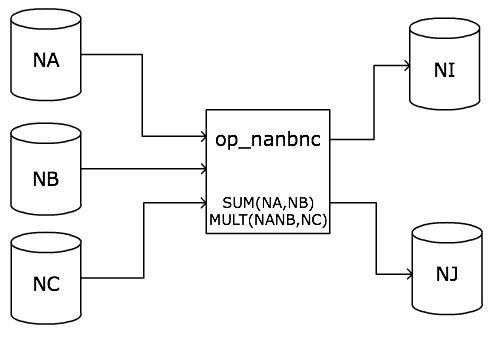
\includegraphics[width=7cm]{images/fig_ex3.jpg}
    \caption{Diagrama do experimento 3}
    \label{fig:ex3}
\end{figure}

Na figura \ref{fig:ex3} ilustra-se um fluxo de trabalho que utiliza como entrada de dados tr�s matrizes: $NA, NB$ e $NC$. O operador aplicado, $op_{\{na,nb,nc\}}$ soma as matrizes $NA$ e $NB$ e a matriz resultante � multiplicada com $NC$.

Apenas um n� ($h_1$) foi utilizado para a execu��o deste experimento. Os detalhes da execu��o est�o descritos na tabela \ref{tab:ex3}.

\begin{table}[ht]
	\centering
	\caption{Resultados do experimento com encadeamento de fluxos}
	\label{tab:ex3}
	\begin{tabular}{llll|l|}
	\hline
	\multicolumn{1}{|c|}{Ordem} & \multicolumn{1}{c|}{Host} & \multicolumn{1}{c|}{Operador} & \multicolumn{1}{c|}{Dados} & \multicolumn{1}{c|}{Tempo (ms)} \\ 
	\hline
	\multicolumn{1}{|c|}{1} & \multicolumn{1}{c|}{$h_1$} & \multicolumn{1}{c|}{SUM,MULT} & \multicolumn{1}{c|}{$NA,NB,NC$} & \multicolumn{1}{r|}{5809} \\ 
	\hline
	\multicolumn{1}{|c|}{2} & \multicolumn{1}{c|}{*} & \multicolumn{1}{c|}{DIFUNDIR} & \multicolumn{1}{c|}{$NI,NJ$} & \multicolumn{1}{r|}{7258} \\ 
	\hline
	\multicolumn{1}{|c|}{3} & \multicolumn{1}{c|}{*} & \multicolumn{1}{c|}{coletor de informa��o} & \multicolumn{1}{c|}{metadados} & \multicolumn{1}{r|}{91} \\ 
	\hline
	\multicolumn{4}{|c|}{tempo de planejamento} & \multicolumn{1}{r|}{1030} \\ 
	\hline
	\multicolumn{4}{|c|}{tempo de tradu��o} & \multicolumn{1}{r|}{580} \\ 
	\hline
	\multicolumn{4}{|c|}{tempo de difus�o} & \multicolumn{1}{r|}{7258} \\ 
	\hline
	\multicolumn{4}{|c|}{tempo processamento} & \multicolumn{1}{r|}{5809} \\ 
	\hline
	\multicolumn{4}{|c|}{tempo total} & \multicolumn{1}{r|}{14790} \\ 
	\hline
	\end{tabular}
\end{table}

\section{Considera��es}
\label{ex-consideracoes}

O principal experimento \ref{ex2} demonstra a capacidade do planejador adaptar o escalonamento de acordo com a situa��o dos recursos. Na primeira execu��o, quando os quatro n�s estavam dispon�veis, o melhor plano foi tra�ado, executando quatro operadores em paralelo $op_{\{h,i\}}$, $ op_{\{e,f\}}$, $op_{\{c,d\}}$ e $op_{\{a,b\}}$, gerando o plano de execu��o com dez passos. Ao trabalhar com um ambiente com um n� parcialmente ocupado, a primeira parte da execu��o foi escalonada com tr�s operadores. Entretanto, outras execu��es paralelas foram alocadas durante o plano deixando-o tamb�m com dez passos.

A utiliza��o da paraleliza��o direta mostra que o ambiente est� preparado para a adequa��o da paraleliza��o por plano, no qual o pr�prio planejador escolhe qual operador e quantos n�s ser�o utilizados para a execu��o de uma determinada tarefa.

No experimento que utiliza m�ltiplas entradas de dados, demonstra-se que sistema � capaz de agregar operadores mais elaborados, que utilizem v�rias opera��es e conjuntos de dados variados.

Os experimentos realizados neste trabalho foram direcionados para a valida��o do modelo (se��o \ref{modelo}). Para isto implementou-se e testou-se as principais funcionalidades para um ambiente de execu��o distribu�da com a gera��o de planos de execu��o por um planejador.

\section[Conclus�o]{Conclus�o}

\begin{frame}
    \frametitle{Conclus�o}
    \begin{itemize}
		\item proposta de um trabalho para execu��o de fluxos de trabalho cient�ficos;
		\item t�cnicas de planejamento:
		\begin{itemize}
			\item tempo de execu��o: estimado fornecido pelo usu�rio;
			\item coeficiente de tempo: execu��es anteriores;
			\item situa��o atual do ambiente distribu�do;
		\end{itemize}
		\item coeficiente de custos: utilizado pelo planejador para criar planos de execu��o;
		\item modulariza��o dos componentes do modelo;
		\item cen�rio flex�vel e expans�vel;
		\item modifica��o do \emph{PeerUnit}: gerenciador de execu��o;
		\item defini��o de um modelo de custos;
		\item uma limita��o do modelo: fluxos c�clicos;
		\begin{itemize}
			\item alternativa parcial: encapsular fluxo de trabalho (m�ltiplas entradas e sa�da de dados);
		\end{itemize}
	\end{itemize}
\end{frame}

\begin{frame}
    \frametitle{Trabalhos Futuros}
    \begin{itemize}
		\item refinamento do \emph{Or�culoDeMetaDados};
		\item utiliza��o de outras m�tricas:
		\begin{itemize}
			\item minimiza��o de gasto de energia;
			\item maximiza��o da utiliza��o de recursos;
		\end{itemize}
		\item m�todo de difus�o inteligente: capaz de analisar o plano e propagar os dados apenas para os n�s que utilizar�o tais dados;
		\item planejador capaz de escolher a melhor implementa��o de um operador para o plano a ser gerado:
		\item paraleliza��o por plano:
		\begin{itemize}
			\item n�o se fixa uma quantidade de n�s para cada fluxo de trabalho;
			\item de acordo com informa��es do \emph{Or�culoDeMetadados} planejador define o n�mero adequado para a paraleliza��o;
			\item necess�ria adapta��o do m�todo de tradu��o (considerar os n�s dispon�veis para cada tarefa);
		\end{itemize}
	\end{itemize}
\end{frame}

\appendix

\chapter{Modelo Inicial Elaborado em JSHOP}
\label{jshop}

Neste ap�ndice apresenta-se a primeira modelagem do problema utilizando a ferramenta JSHOP \cite{Ilghami2006}.

Os c�digos \ref{jshopproblem} e \ref{jshopdomain} apresentam os arquivos de problema e dom�nio modelados.

\UFPRcode{Java}{jshopproblem}{Problema elaborado em JSHOP}{codes/jshop_problem.txt}

Nota-se que a elabora��o do arquivo de problema � muito semelhante a um problema elaborado na linguagem PDDL. O problema em quest�o utiliza tr�s tarefas. A tarefa $A$ e $B$ s�o dependentes do dado $D_1$, e geram como sa�da $D_{21}$ e $D_{22}$ respectivamente. a tarefa $C$ utiliza como entrada $D_{21}$ e $D_{22}$ e gera $D_3$ que tamb�m � o objetivo. Est�o dispon�veis tr�s n�s ($H1, H2$ e $H3$).

Como o JSHOP trabalha com um sistema hier�rquico de decomposi��o de tarefas, solicita-se que cada resolu��o \emph{doplan} seja executada separadamente. Ainda foi utilizado um m�todo para finaliza��o de cada uma das tarefas (caso ainda n�o tenha sido finalizada pela estrutura recursiva).

\UFPRcode{Java}{jshopdomain}{Dom�nio elaborado em JSHOP}{codes/jshop_domain.txt}

Como dom�nio do problema descreve-se a��es de inicializa��o e finaliza��o de tarefa. O m�todo \emph{doplan} � o m�todo principal. Ele invoca os demais m�todos ou ele pr�prio recursivamente caso seja necess�rio. O m�todo \emph{resolve-all} � utilizado para resolver todas as depend�ncias de uma tarefa que necessita dos dados para sua execu��o. O m�todo \emph{finish-task} � invocado e termina uma tarefa com o operador \emph{end-task} caso ela ainda esteja em execu��o.

A figura \ref{fig:jshopdec} mostra a decomposi��o utilizada para a gera��o do plano.

\begin{figure}[!htb]
    \centering
    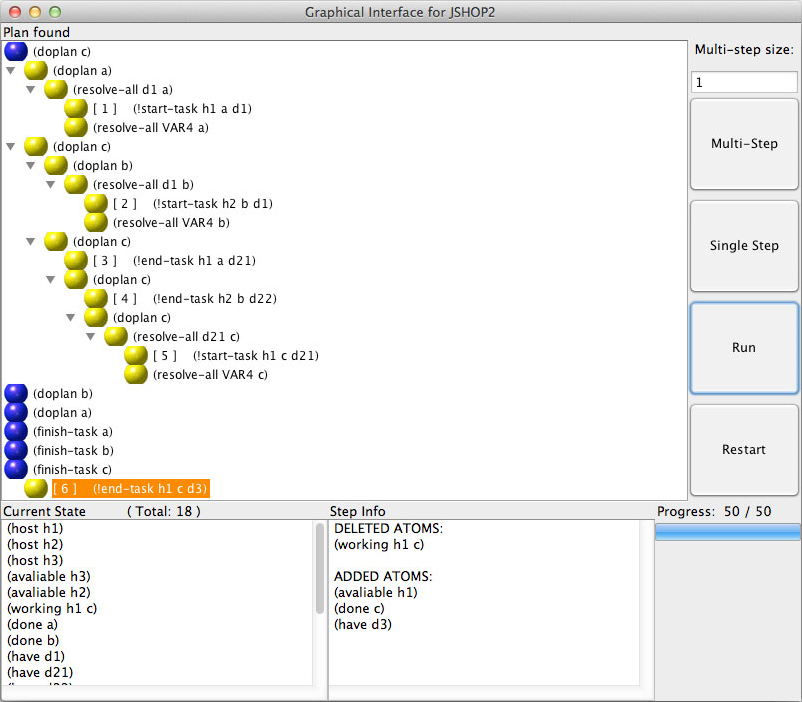
\includegraphics[width=10cm]{images/fig_jshop.jpg}
    \caption{Decomposi��o de a��es no JSHOP}
    \label{fig:jshopdec}
\end{figure}

O c�digo \ref{jshopresult} mostra o resultado obtido.

\UFPRcode{Java}{jshopresult}{Plano de a��es retornado pelo JSHOP}{codes/jshop_result.txt}

Com a decomposi��o das tarefas conseguiu-se inicialmente um plano de execu��o aceit�vel entretanto � f�cil observar que as a��es $1$ e $2$ poderiam ser executadas de forma paralela, visto que cada uma delas utiliza um n� diferente. Esta foi a principal motiva��o para a utiliza��o de um planejador capaz de gerar planos paralelos.
    %%%%%%%%%%%%%%%%%%%%%%%%%%%%%%%%%%%%%%%%%%%%%%%%%
    % R E C U R S O S   C O M P U T A C I O N A I S %
    %%%%%%%%%%%%%%%%%%%%%%%%%%%%%%%%%%%%%%%%%%%%%%%%%

    \UTFPRchapter[cap:recursos]{RECURSOS COMPUTACIONAIS}

    Os recursos computacionais necess�rios s�o divididos entre:
    recursos dispon�veis para desenvolvimento e recursos
    necess�rios para utiliza��o descritos nas Se��es
    \ref{sec:recursosdeselvolvimento} e \ref{sec:recursosutilizacao}
    respectivamente.

    \UTFPRsection[sec:recursosdeselvolvimento]{RECURSOS DISPON�VEIS PARA DESENVOLVIMENTO}

    \UTFPRsubsection{Recursos de Hardware}

        \begin{enumerate}

        \item Microcomputador Desktop:

        \begin{enumerate}
            \item[a)] \emph{Processador:} AMD Athlon(tm) XP 2700+ (2.16 GHz);
            \item[b)] \emph{Mem�ria:} 512 MB;
            \item[c)] \emph{Armazenamento:} 120GB + 40GB.
        \end{enumerate}

        \item Microcomputador Notebook:

        \begin{enumerate}
            \item[a)] \emph{Modelo:} HP Pavilion dv1040;
            \item[b)] \emph{Processador:} Pentium M Centrino  (1.7 GHz);
            \item[c)] \emph{Mem�ria:} 512 MB;
            \item[d)] \emph{Armazenamento:} 60GB.
        \end{enumerate}

        \end{enumerate}

    \UTFPRsubsection{Recursos de \emph{Software}}

        \begin{enumerate}

        \item Sistemas Operacionais:

        \begin{enumerate}

            \item[a)] \emph{Windows XP Professional Edition SP2 PT-BR}:
            Sistema operacional utilizado com o
            microcomputador \emph{desktop};

            \item[b)] \emph{Windows XP Home Edition SP2 EN-US}:
            Sistema operacional utilizado com o
            microcomputador \emph{notebook}.

        \end{enumerate}

        \item Outros \emph{Softwares}:

        \begin{enumerate}
            \item[a)] \emph{Adobe Photoshop CS2}:
            Necess�rio para a constru��o dos \emph{layouts} (\emph{design}) do
            sistema;

            \item[b)] \emph{Adobe Acrobat Reader Professional 7.0}:
            Necess�rio para visualiza��o e altera��o
            do \UTFPRsigla{PDF}{\emph{Portable Document Format}} referente
            � monografia;

            \item[c)] \emph{Apache HTTP Server 1.3.33}:
            Servidor HTTP com suporte a linguagem PHP;

            \item[d)] \emph{Macromedia Dreamweaver 8.0}:
            Utilizado para a codifica��o e design do sistema;

            \item[e)] \emph{Visual Paradigm vers�o 5.2}:
            Utilizado para constru��o dos diagramas UML;

            \item[f)] \emph{Mozilla Firefox vers�o 1.5.0.5}:
            Navegador compat�vel com as especifica��es HTML 4.01,
            CSS 2, e possui suporte a JavaScript. Utilizado para
            testes no sistema;

            \item[g)] \emph{Internet Explorer 7.0}:
            Navegador compat�vel com as especifica��es HTML 4.01,
            CSS 2, e possui suporte a JavaScript. Utilizado para
            testes no sistema;

            \item[h)] \emph{winEdit 5.4}: Programa
            utilizado para codifica��o da monografia em \LaTeX;

            \item[i)] \emph{PostGreSQL 8.0.1}: Banco de
            dados utilizados neste trabalho;

            \item[j)] \emph{pgAdmin 1.4.2}: Ferramenta
            para gerenciamento do banco de dados PostGreSQL;

            \item[k)] \emph{ERwin 4.0}: Ferramenta para
            cria��o dos diagramas de entidades e relacionamentos;

            \item[l)] \emph{MiKTeX 2.5}: Compilador
            \LaTeX{} para Windows;

            \item[m)] \emph{PHP 5.1.4}: Linguagem de
            programa��o utilizada neste trabalho;


            \item[n)] \emph{LaTable 0.7.2}: Ferramenta
            para cria��o de tabelas;

            \item[o)] \emph{yEd Graph Editor 2.4.2.2}: Ferramenta
            para cria��o dos grafos.

        \end{enumerate}

        \end{enumerate}

    \UTFPRsection[sec:recursosutilizacao]{RECURSOS NECESS�RIOS PARA UTILIZA��O}

    \UTFPRsubsection{Usu�rio}

        Para utilizar o sistema, o usu�rio dever� possuir um microcomputador
        conectado a Internet com um navegador compat�vel com as
        especifica��es HTML 4.01, CSS 2 com suporte a
        JavaScript.

    \UTFPRsubsection{\emph{Website} Hospedeiro}

        O sistema elaborado, poder� ser implantado em \emph{websites} comuns
        que contemplem determinadas restri��es, tais como:

        \begin{itemize}
            \item O \emph{website} deve estar rodando em um navegador
                compat�vel com as especifica��es HTML 4.01, CSS 2, e
                deve possuir suporte a JavaScript;

            \item O \emph{website} deve suportar a linguagem de programa��o
            PHP;

            \item O \emph{website} deve possuir suporte ao banco de dados
            PostGreSQL 8.1, com disponibilidade de um banco de dados para o sistema a ser
            implantado.

        \end{itemize}

\chapter{Arquivos de Planejamento}
\label{plan-files}

Neste ap�ndice apresenta-se exemplos de c�digos que representam os arquivos de dom�nio (se��o \ref{ap-dominio}), problema (se��o \ref{ap-problema}) e o plano gerado (se��o \ref{ap-plano}).

Os arquivos apresentados foram gerados automaticamente pelo tradutor que � apresentado em \ref{ap-tradutor}. O m�todo de tradu��o � detalhado em \ref{tradutor}.

\section{Dom�nio}
\label{ap-dominio}

\UFPRcode{Java}{rec_domain}{C�digo representa o dom�nio de um problema em PDDL}{codes/rec_domain.txt}

\section{Problema}
\label{ap-problema}

\UFPRcode{Java}{rec_problem}{C�digo representa um problema em PDDL}{codes/rec_problem.txt}

\section{Plano Gerado}
\label{ap-plano}

Nota-se que o plano gerado pela execu��o do plaejador \emph{CRIKEY} (se��o \ref{crikey}) apresenta a��es paralelas. A a��o $0.01$ � formada por duas instru��es, bem como a a��o $0.02$.

\UFPRcode{Java}{rec_plan}{Sa�da que representa um plano gerado pelo \emph{CRIKEY}}{codes/rec_plan.txt}

\chapter{Descri��o dos Componentes}
\label{components-description}

Neste ap�ndice apresenta-se a descri��o dos componentes apresentados Vis�o Detalhada do Sistema (se��o \ref{visao-detalhada}), bem como a descri��o dos componentes auxiliares utilizados para a implementa��o do sistema. Cada componente representa uma classe Java.

A organiza��o dos componentes pode ser observada na figura \ref{fig:components}.

\begin{figure}[!htb]
   \centering
    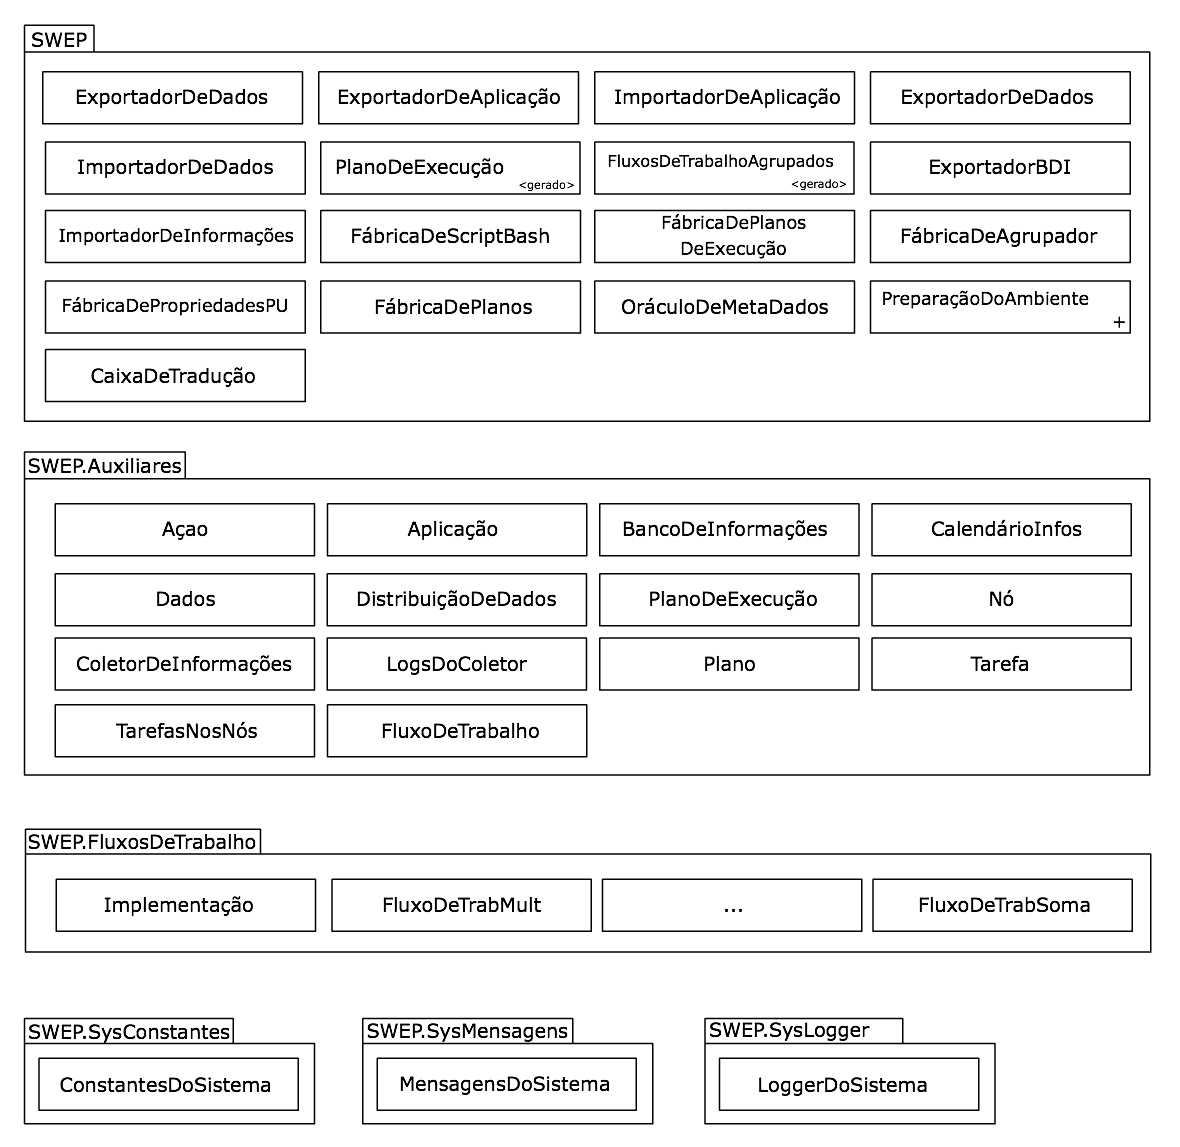
\includegraphics[width=14cm]{images/fig_sys_components.jpg}
    \caption{Componentes do sistema}
    \label{fig:components}
\end{figure}

A tabela \ref{tab:descriptions} mostra a descri��o de cada um dos componentes.

\begin{table}[!htb]
	\caption{Descri��o dos componentes.}
	\label{tab:descriptions}
	\scriptsize
	\begin{longtable}{|l|l|}
		\hline
		\multicolumn{2}{|c|}{SWEP} \\ 
		\hline
		ExportadorDeA��es & Exporta as a��es para gera��o de um plano de execu��o. \\ 
		\hline
		ExportadorDeAplica��o & Exporta as informa��es da aplica��o. \\ 
		\hline
		ImportadorDeAplica��o & Importa as informa��es da aplica��o. \\ 
		\hline
		ExportadorDeDados & Exporta os dados para um formato aceit�vel pelo sistema. \\ 
		\hline
		ImportadorDeDados & Importa os dados. \\ 
		\hline
		PlanoDeExecu��o & � um plano de execu��o (Gerado automaticamente). \\ 
		\hline
		FluxosDeTrabalhoAgrupados & Jun��o de todos os operadores dipon�veis (Gerado automaticamente). \\ 
		\hline
		ExportadorBDI & Exporta uma base de dados do coletor de informa��es. \\ 
		\hline
		ImportadorDeInforma��es & Importa uma base de dados do coletor de informa��es. \\ 
		\hline
		F�bricaDeScriptBash & Cria um arquivo bash para a execu��o do ambiente. \\ 
		\hline
		F�bricaDePlanosDeExecu��o & Cria um plano de execu��o com base na a��es exportadas. \\ 
		\hline
		F�bricaDeAgrupador & Cria o arquivo JoinWorkFlow que reune todos os operadores dispon�veis. \\ 
		\hline
		F�bricaDePropriedadePU & Cria  o arquivo de propriedades do gerenciador de execu��o com as informa��es do sistema. \\ 
		\hline
		F�bricaDePlanos & Invoca o planejador e gera um plano. \\ 
		\hline
		Or�culoDeMetaDados & Retorna informa��es referente aos n�s. \\ 
		\hline
		Prepara��oDoAmbiente & Arquivo execut�vel que coordena a execu��o do ambiente. \\ 
		\hline
		CaixaDeTradu��o & � respons�vel pela tradu��o das informa��es do sistema nos arquivos PDDL. \\ 
		\hline
		\multicolumn{2}{|c|}{Auxiliares} \\ 
		\hline
		A��o & Representa uma a��o. \\ 
		\hline
		Aplica��o & Representa a aplica��o. \\ 
		\hline
		BancoDeInforma��es & Representa uma base de coletores de informa��o. \\ 
		\hline
		Calend�rioInfos & Retorna informa��es de data e hora. \\ 
		\hline
		Dados & Representa uma cole��o de dados. \\ 
		\hline
		Distribui��oDeDados & Representa um sistema de paraleliza��o de dados simplista. \\ 
		\hline
		PlanoDeExecu��o & Representa um plano de execu��o. \\ 
		\hline
		N� & Representa um n�. \\ 
		\hline
		ColetorDeInforma��es & Representa um coletor de informa��o em um n�. \\ 
		\hline
		LogsDoColetor & Representa um coletor de log de tarefas executadas. \\ 
		\hline
		Plano & Representa um plano. \\ 
		\hline
		Tarefa & Representa uma tarefa. \\ 
		\hline
		FluxoDeTrabalho & Representa quais tarefas foram executadas por cada n�. \\ 
		\hline
		WorkFlow & Representa um fluxo de trabalho. \\ 
		\hline
		\multicolumn{2}{|c|}{Fluxos de Trabalho} \\ 
		\hline
		Implementa��o & � a base para implementa��o dos demais operadores. \\ 
		\hline
		FLuxoDeTrabMult & Representa um operador que executa a multiplica��o de matrizes. \\ 
		\hline
		FluxoDeTrabSoma & Representa um operador que executa a soma de matrizes. \\ 
		\hline
		\multicolumn{2}{|c|}{SysConstantes} \\ 
		\hline
		ConstantesDoSistema & Armazena as constantes do sistema. \\ 
		\hline
		\multicolumn{2}{|c|}{SysMensagens} \\ 
		\hline
		MensagensDoSistema & Armazena as mensagens do sistema. \\ 
		\hline
		\multicolumn{2}{|c|}{SysLogger} \\ 
		\hline
		LoggerDoSistema & Cont�m esquema de gera��o de logs do sistema. \\ 
		\hline
	\end{longtable}
	\normalsize
\end{table}
\chapter{Arquivo de Configura��o do PeerUnit}
\label{peer-unit-file}

Neste ap�ndice apresenta-se o arquivo de configura��o do ambiente de execu��o \emph{PeerUnit} descrito na se��o \ref{peerunit}.

\UFPRlongcode{Java}{peerunit_file}{Arquivo de configura��o do PeerUnit}{codes/peerunit.properties}
\chapter{C�digos Fonte}
\label{source-codes}

Neste ap�ndice apresenta-se exemplos de c�digos fonte utilizados para na implementa��o do sistema.

\section{Chamada do Planejador}
\label{ap-chamada-planejador}

O c�digo \ref{source_plan} mostra o arquivo que corresponde ao componente \emph{F�bricaDePlanos}. Nesse componente o m�todo \emph{doMakePlan()} � que invoca o planejador \emph{Crikey}. O sistema aguarda at� que o arquivo de sa�da seja gravado, e em seguida o utiliza para a gera��o do arquivo contendo as a��es.

\UFPRlongcode{Java}{source_plan}{Exemplo que invoca o planejador}{codes/MakePlan.java}

\section{Plano de Execu��o}
\label{ap-plano-execucao}

O c�digo \ref{execution_plab} exemplifica um plano de execu��o gerado automaticamente a partir do arquivo de a��es gerado pelo planejador.

\UFPRlongcode{Java}{execution_plab}{Exemplo de um plano de execu��o}{codes/ExecutionPlanGenerated.java}

\section{Fluxo de Trabalho de Exemplo}
\label{ap-fluxo-exemplo}

Apresenta-se um exemplo da implementa��o de um operador. O c�digo \ref{implementation} apresenta o componente que � herdado pelos operadores. O c�digo \ref{source_workflow} mostra a implementa��o de um operador para soma de matrizes.

\subsection{Implementa��o Base}
\label{ap-implementation}

\UFPRlongcode{Java}{implementation}{Implementa��o b�sica para fluxos de trabalho}{codes/Implementation.java}

\subsection{Fluxo de Trabalho para Soma de Matrizes}
\label{ap-workflow-sum}

\UFPRlongcode{Java}{source_workflow}{Fluxo de trabalho para soma de matrizes}{codes/WorkflowSumVet.java}

\section{Tradutor}
\label{ap-tradutor}

O c�digo \ref{source_translation} demonstra todo o modelo detalhado na se��o \ref{tradutor}.

\UFPRlongcode{Java}{source_translation}{C�digo que faz a tradu��o do sistema para os arquivos PDDL}{codes/WorkflowSumVet.java}


%%%%%%%%%%%%%%%%
% BIBLIOGRAFIA %
%%%%%%%%%%%%%%%%

\bibliographystyle{bst/bibstyle}
\bibliography{bib/bibliografia}

\addcontentsline{toc}{chapter}{\MakeUppercase{Bibliografia}}

\singlespacing
\makecapadissertacao

\end{document}